%%sudo apt-get install texlive-lang-spanish

\documentclass[spanish]{report}
\setcounter{secnumdepth}{1}
\usepackage[spanish]{babel}
\selectlanguage{spanish}
\usepackage[utf8]{inputenc}
\usepackage{hyperref}
\usepackage{amssymb}
%%\usepackage{cite}
\usepackage{graphicx}
\usepackage{float}
%%\usepackage[margin=1cm]{caption}
\usepackage{caption}
\usepackage[backend=biber]{biblatex}
\usepackage{amsmath}
%%sudo apt-get install texlive-science
\usepackage{algorithm,algorithmic}
\usepackage[bottom]{footmisc}
\usepackage{tocloft}
\usepackage{blindtext}
%%sudo apt-get install texlive-fonts-extra 
\usepackage{ dsfont }


\setlength{\cftbeforetoctitleskip}{0pt}
\setlength{\cftaftertoctitleskip}{0pt}
\DeclareMathOperator*{\argmax}{argmax} % thin space, limits underneath in displays


\pagestyle{headings}	

\makeatletter
\renewcommand{\ALG@name}{Algoritmo}
\makeatother

\renewcommand{\baselinestretch}{1.5}
\addbibresource{tesina.bib}
\selectlanguage{spanish}

\begin{document}

\begin{titlepage}

\begin{center}
\huge{Generación de imágenes con redes neuronales profundas a partir del enfoque en objetos.}

\vfill

\large
Tesina de grado

Licenciatura en Ciencias de la Computación.

\vspace{0.5cm}
\[

\includegraphics[width=100px]{logo-unr.jpg}
\]
\normalsize
Facultad de Ciencias Exactas, Ingeniería y Agrimensura

Universidad Nacional de Rosario
\end{center}

\vfill

\begin{center}
\large

Nicolás Antinori

\vspace{0.5cm}

\textit{Director}

Guillermo Luis Grinblat

\end{center}

\end{titlepage}
\newpage

\begin{abstract}

Las redes neuronales profundas convolucionales han demostrado ser muy eficaces en aprender conceptos complejos con imágenes y han desempeñado un papel excelente en tareas tales como reconocimiento de objetos. En el último tiempo surgió un nuevo tipo de redes llamadas Generative Adversarial Networks (GANs) las cuales son muy útiles para la generación de imágenes, donde, a partir de una muestra aleatoria de distribución simple, se la transforma en una muestra que se aproxima a la distribución de un dataset.

Basándonos en estudios que demuestran la importancia del movimiento en el reconocimiento de formas y patrones que definen un objeto en una escena, se propone extraer la información provista por el movimiento en distintos fotogramas de un video e insertarla como un canal extra en las imágenes que conforman los datasets de entrenamiento.

La información adquirida a partir del análisis automático de movimiento en fotogramas consecutivos es la separación entre el fondo y objetos en el primer plano de una escena. A partir de esta separación, se hace foco en los objetos que están en primer plano y se adiciona dicha información como un canal extra en cada imagen del dataset. Dado que el análisis automático presenta imperfecciones, también se utilizará un dataset con imágenes segmentadas por humanos, el cual representa las condiciones ideales con respecto al enfoque de objetos.

El objetivo de este trabajo es utilizar las segmentaciones anteriormente nombradas para tratar de obtener mejoras en la generación de imágenes con datasets de mucha variabilidad. Para tener un punto de comparación, las redes se entrenan con dos versiones de cada uno de los datasets: uno conformado con imágenes con los tres canales convencionales (R, G, B) y el mismo con el canal adicional correspondiente en cada imagen.

Los resultados obtenidos parecen sugerir que el canal extra mejora la generación de imágenes, siendo esta mejoría muy dependiente de la calidad de las segmentaciones utilizadas.


\end{abstract}

\newpage

\huge\textbf{Agradecimientos\\}

\normalsize
Quiero agradecer enormemente al equipo de investigación de Machine Learning y en especial Guille por todo el tiempo, dedicación y paciencia que me brindó a lo largo de esta tesina.

A Matías Chomicki, Exequiel Rivas y Matías Olocco, que fueron mis primeros mentores y los que me inspiraron a seguir mi camino en computación.

A los grandes amigos que hice en la facultad, Adriel, Alejo, Berta, Eze, Javo, Leus, Lulo, Mel y Nati, por las largas horas de estudio y los buenos momentos fuera de la facultad.

A mis amigos de toda la vida, Ariel, Carlitos, Lalo, Lulo, David, Jere, Maxi y Tony por estar siempre y aguantar el clásico ``no puedo, tengo que estudiar''.

A mi novia, Mel, por todo el apoyo emocional, el cariño y la paciencia que me tuvo a lo largo de todo este proceso.

Y por último, pero no por eso menos importante a mi familia, que sin su acompañamiento y ayuda incondicional me hubiese sido imposible dedicarme a esto. A mi mamá Patricia, a mi papá Angel, a mi hermano Lucas y a mi abuela Nilda. Este trabajo es para ellos.

\newpage


\tableofcontents

\newpage


\chapter{Introducción}

\section{Problemática}
En la actualidad, para la generación de muestras a partir de observaciones se utilizan las Generative Adversarial Networks (GAN) \cite{goodfellow_generative_2014} que son una clase de algoritmos de inteligencia artificial implementados por un sistema de dos redes neuronales que compiten mutuamente en un juego de suma cero.

Las GANs suelen funcionar mejor cuando el aprendizaje es supervisado (en este contexto, se dice que es supervisado cuando la red llamada ``discriminador'' es entrenada con etiquetas de clase con dos objetivos: detectar si la imagen proviene del dataset de entrenamiento o fue producida por la red llamada ``generador'' y asignarle una etiqueta de clase. La red llamada ``generador'' es entrenada con el objetivo de poder sintetizar una imagen a partir de una etiqueta), y más aún con datasets restringidos como el caso de CelebA, un dataset formado por rostros de celebridades \cite{celebA}. En el caso de datasets mucho más generales (como por ejemplo ImageNet \cite{imagenet_cvpr09}) la red genera imágenes que, aunque suelen tener texturas muy bien logradas, a simple vista parecen pertenecer a alguna clase del dataset con la que fue entrenada pero en detalle le falta o le sobran características claves de la misma (por ejemplo, para la clase perro, un torso con 5 patas y un hocico). Esto mismo empeora en el caso no supervisado.

\section{Motivación y objetivos}

Existen estudios \cite{visual_parsing} que demuestran que tanto infantes, como gente que recuperó la visión, tienden a sobresegmentar objetos cuando los ven de forma estática, pero pueden diferenciarlos correctamente cuando estos están en movimiento. En un video, los píxeles correspondientes a un objeto suelen moverse de forma diferente e independientemente de los píxeles que forman el fondo. Teniendo en cuenta esto, podemos obtener información de cómo se puede estar moviendo un objeto utilizando algunos fotogramas del video, para segmentarlo del fondo y enfocarse en el mismo.

Para la experimentación, este trabajo hace enfoque en la ampliación de los datasets agregando información de segmentación obtenida a través de distintos procesos que se describirán en el Capítulo 3, más que en la modificación de las GAN. Las GAN serán alteradas de forma mínima para poder utilizar datasets con información de segmentación agregada.

El objetivo de este trabajo es investigar el efecto que puede tener el uso de la información de segmentación sobre una GAN entrenada de manera no supervisada para evaluar si ésta puede aprender características más fuertes y más definidas y en consecuencia, generar mejores imágenes.

\section{Organización del trabajo}

\noindent Este trabajo está organizado de la siguiente manera: 
~\\

El Capítulo 2, \textit{Conceptos generales}, explica todos los conceptos del aprendizaje automatizado necesarios para entender esta tesina.
~\\

El Capítulo 3, \textit{Experimentos}, expone los distintos datasets utilizados, su estructura, cómo fueron generados y procesados para su uso en este trabajo. Además expone los resultados de la experimentación y un análisis de los mismos.
~\\

El Capítulo 4, \textit{Conclusiones y trabajos futuros}, muestra las conclusiones obtenidas de este trabajo y provee posibles proyectos futuros.
~\\

\chapter{Conceptos generales}

\section{Aprendizaje automático}

El aprendizaje automático (Machine Learning) es una rama de las ciencias de la computación que se dedica a estudiar técnicas que permitan a una computadora aprender a realizar una tarea sin haber sido específicamente programada para la misma. 

Se dice que un programa de computadora aprende de la experiencia \textit{E} con respecto a algún tipo de tarea \textit{T} con una medición de eficacia \textit{P}, si su eficacia en la tarea \textit{T} medida con \textit{P} mejora con la experiencia \textit{E} \cite{Mitchell97a}.

El objetivo de todo proceso de aprendizaje automático es encontrar una función hipótesis

\[ h: X \rightarrow Y, \]

\noindent que mejor aproxime una función objetivo

\[ f: X \rightarrow Y, \]

\noindent la cual es desconocida y es la que modela de forma óptima el problema que se está tratando.

Es común tener tres conjuntos de datos para entrenar algoritmos de aprendizaje automatizado. Por un lado, se tienen los datos de entrenamiento, los cuales son la fuente principal de conocimiento y es de donde el algoritmo va aprendiendo a modelar el problema. Por otro lado, están los datos de validación que suelen ser un subconjunto apartado de los datos de entrenamiento y se utilizan tanto para ajustar los parámetros del algoritmo, como así también para medir y prevenir el sobreajuste (Sección \ref{sobreajuste}). Por último, existen los datos de testing. Normalmente suelen estar completamente aislados de los datos de entrenamiento y validación. Se utilizan para medir el error de generalización de un algoritmo completamente entrenado. No es necesario que los tres tipos de conjuntos estén siempre presentes en todos los problemas que se quieran modelar, esto depende de lo que se quiere medir.

\subsection{Aprendizaje supervisado y no supervisado}


El aprendizaje supervisado consiste en utilizar un conjunto de entrenamiento con datos etiquetados. Un elemento de dicho conjunto es una tupla $(x, y) \in X \times Y$, donde $x$ es el dato de entrada e $y$ es la etiqueta, representando el valor de salida que se espera encontrar para $x$.

El aprendizaje no supervisado no posee etiquetas de clasificación en sus datos de entrenamiento, sino que deja que el algoritmo aprenda a modelar de manera automática el problema tratado.


\subsection{Sobreajuste}\label{sobreajuste}

Los datos de entrenamiento no siempre son perfectos. Puede suceder que no se tenga un conjunto lo suficientemente grande como para poseer una muestra representativa de lo que se quiere modelar o que el mismo contenga muchos elementos corruptos. El problema con este escenario es que lleva al algoritmo a aprender características muy específicas sobre los datos de entrenamiento, perdiendo así la capacidad de generalizar sobre todo el conjunto de entrada Este fenómeno se puede observar en la Figura \ref{fig:graphsobreajuste}.


\begin{figure}[h!]
  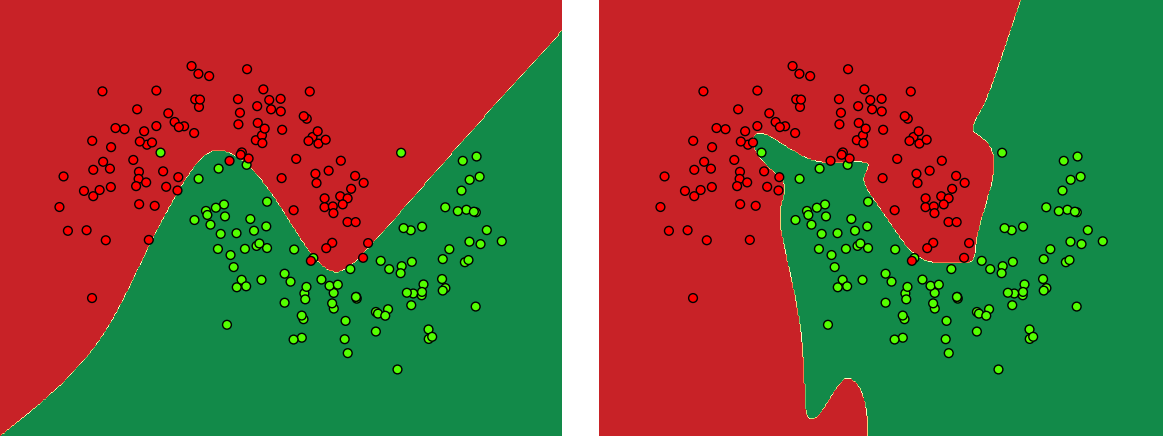
\includegraphics[width=\linewidth]{overfit_ejemplos.png}
  \caption{Entrenamiento de una red neuronal sobre el dataset ``two moons'' \cite{scikitLearn}. A la izquierda, el resultado del entrenamiento en 200 iteraciones. A la derecha, el resultado del entrenamiento en 2000 iteraciones. Se puede observar cómo en esta última el modelo se sobreajustó, tomando regiones rojas como si fuesen verdes, debido al ruido contenido en los datos.}
  \label{fig:graphsobreajuste}
\end{figure}


\begin{figure}[H]
\centering
 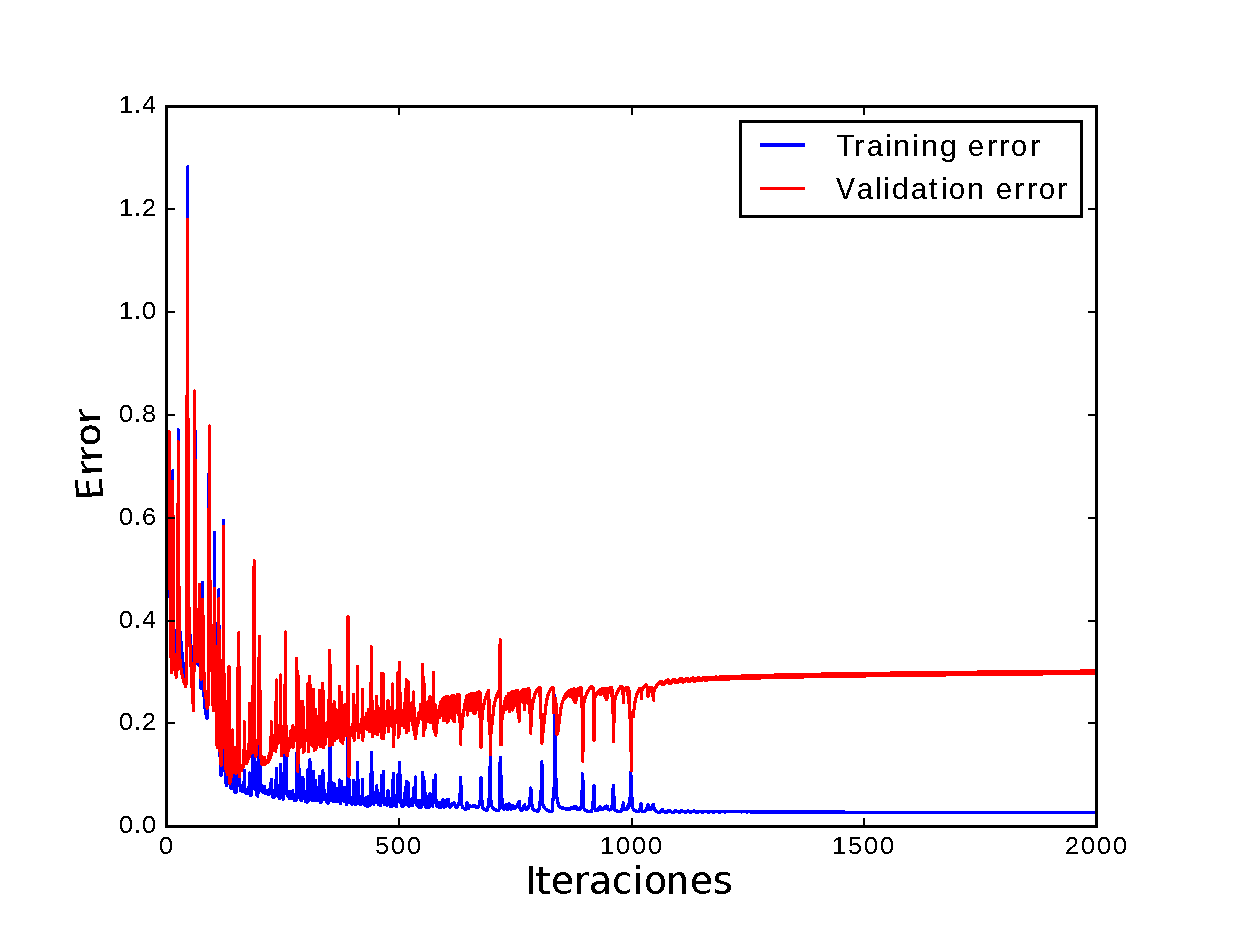
\includegraphics[width=\linewidth]{overfitplot.eps}
  \caption{Evolución del entrenamiento de una red neuronal para el reconocimiento de clases. Entrenada con el dataset ``two moons''.}
  \label{fig:overfitplot}
\end{figure}


Más formalmente, dado un espacio de funciones hipótesis $H$, se dice que una función $h \in H$ sobreajusta los datos de entrenamiento si existe una función $h' \in H$, tal que $h$ tiene un menor error que $h'$ en los datos de entrenamiento pero $h'$ tiene un menor error que $h$ sobre todo el espacio de entrada.
\newline

Una forma de detectar el sobreajuste es evaluar lo aprendido hasta el momento contra un conjunto de validación. Como se puede observar en la Figura \ref{fig:overfitplot}, a medida que avanzan las iteraciones, el error de entrenamiento baja mientras que el error de validación se incrementa, perdiendo así cada vez más generalidad sobre lo aprendido.


\subsection{Sesgo inductivo}

El \textit{sesgo inductivo} es el conjunto de suposiciones que el algoritmo de aprendizaje utiliza para predecir resultados de entradas que nunca vio.

La finalidad del entrenamiento es encontrar una función hipótesis que nos ayude a predecir o generar una cierta salida a partir de un conjunto de entrada definido. El algoritmo es entrenado con una cantidad finita de ejemplos que muestra la relación entre las entradas y las salidas. Luego del entrenamiento, es esperable que se pueda predecir o generar una salida adecuada incluso para una entrada nunca vista en la etapa de aprendizaje.

Sin suposiciones adicionales, la inducción en datos nunca antes vistos no sería posible dada las (posiblemente) infinitas formas que existen de generalizar el problema tratado.

Un ejemplo clásico del sesgo inductivo es el de la navaja de Occam: \textit{Debe preferirse la hipótesis más simple consistente con los datos}. Donde consistente se refiere a que la hipótesis nos da resultados correctos para todas las entradas de ejemplo que se le han dado al algoritmo.

\newpage


\section{Redes Neuronales}

Las redes neuronales artificiales (RNAs)\cite{Mitchell97a} son un método de aprendizaje automatizado que provee un enfoque robusto para aproximar funciones objetivo a valores reales, discretos y vectoriales. 

Están conformadas por neuronas artificiales (Figura \ref{fig:neurona_artificial}). Cada neurona es una unidad de cómputo, la cual tiene como entrada un vector de valores con los que calcula una combinación lineal y obtiene como salida un valor, representando el grado de activación de la misma. 

Más formalmente, sean $x_1, x_2, ..., x_n$ las entradas de una neurona, entonces su valor de salida está dado por:\begin{equation}
o = f(\sum_{i=0}^{n}{w_i x_i}),
\end{equation}

\noindent donde $f$ es conocida como la función de activación y cada $w_i$ es un valor real llamado peso, que determina la contribución de la entrada $x_i$ a la salida de la neurona. Nótese que la suma comienza en 0 y no en 1. Fijando $x_0=1$ tenemos que cada neurona computa un peso extra llamado \textit{bias} (sesgo), el cual nos da un umbral para su activación. 

\begin{figure}[H]
\centering
 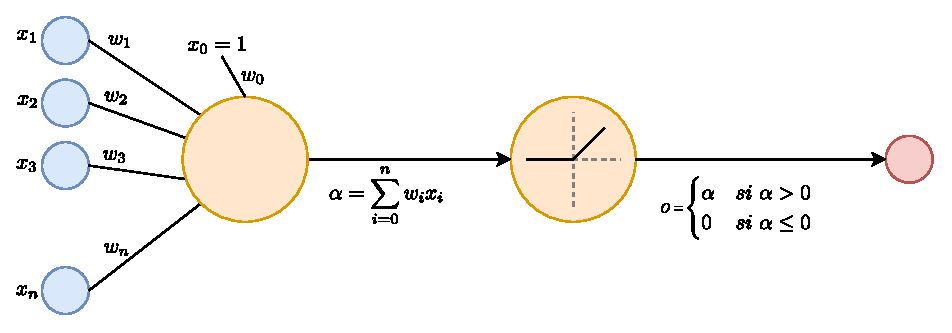
\includegraphics[width=\linewidth]{neurona.eps}
 \caption{Representación de una neurona artificial con entradas $x_i$, pesos $w_i$ con $i \in [1, .., n]$, bias $w_0$ y función de activación ReLU.}
 \label{fig:neurona_artificial}
\end{figure}

\newpage
La función de activación tiene el propósito de otorgarle no-linearidad a la neurona. Existen varias funciones de activación comúnmente utilizadas\label{activaciones}:


\begin{itemize}
\item Sigmoidea: $f(x) = \dfrac{1}{1+e^{x}}$
\item Tangente hiperbólica: $f(x) = \dfrac{e^{x}-e^{-x}}{e^{x}+e^{-x}}$
\item ReLU: 
$
f(x) =  \begin{cases}
		    x & si~x > 0 \\
			0 & si~x \leq 0
		\end{cases}
$

\item Leaky ReLU: 
$
f(x) =  \begin{cases}
		    x & si~x > 0 \\
			0.01 & si~x \leq 0
		\end{cases}
$				
\end{itemize}
~\newline

Las RNAs están generalmente organizadas en capas (Figura \ref{fig:red_neuronal_capas}), donde cada una de ellas contiene un número de neuronas  conveniente al problema que se esté tratando. Las neuronas pertenecientes a una misma capa no están conectadas entre ellas, pero si están interconectadas con las neuronas de sus capas adyacentes. Más formalmente, una RNA es un conjunto de neuronas que forman un grafo acíclico, donde la salida de algunas neuronas sirven de entrada para neuronas de la capa subsiguiente.

Las capas se organizan de la siguiente manera. La primer capa es de entrada, tiene como función recibir los valores a procesar. Luego, una o varias capas intermedias, llamadas \textit{capas ocultas} y por último la capa de salida, que es donde se presentan los resultados obtenidos.

El objetivo de entrenar una RNA es obtener para cada una de las neuronas un vector de pesos $\vec{w}^{\,} = (w_0, w_1, ..., w_n)$ que minimice lo más posible el error de salida de la red.


\begin{figure}[H]
\centering
 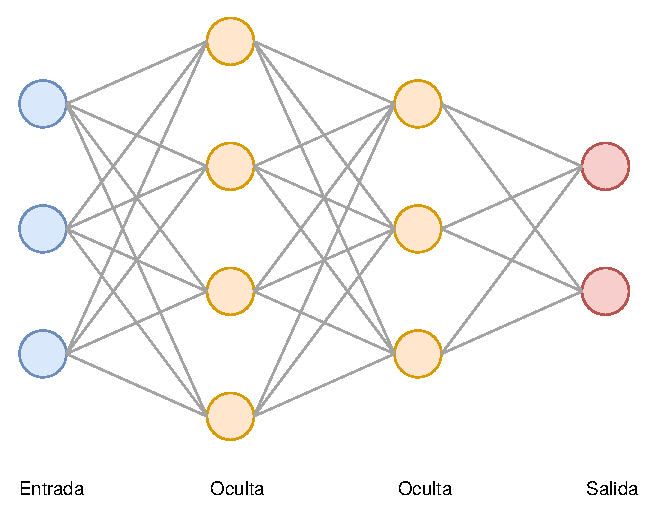
\includegraphics[width=\linewidth]{RNA.eps}
  \caption{Representación de una red neuronal. A la izquierda, la capa de entrada con tres neuronas. En el medio, las capas ocultas con cuatro y tres neuronas respectivamente. Por último, la capa de salida con dos neuronas.}
   \label{fig:red_neuronal_capas}
\end{figure}

%%\subsubsection{Entrenando una red}

%%Para entrenar una RNA se utiliza un método de que se conoce como refinamiento iterativo. Se empieza con un conjunto de pesos aleatorios y en cada iteración se van ajustando los mismos para que el error de salida vaya disminuyendo. Para lograr esto se utiliza una ténica llamada \textit{descenso por el gradiente}. Normalmente el error es medido con una función llamada "función de pérdida" (loss function) que nos da un parámetro de cuán alejados estamos.  


\subsubsection{Descenso por el gradiente}

Consideremos el caso de entrenar sólo una neurona. En esta situación el problema se reduce a aprender el vector de pesos $\vec{w}^{\,} = (w_0, w_1, ..., w_n)$ que hace que la neurona produzca una salida correcta para cada ejemplo de entrenamiento.

Para entrenar esta neurona se puede utilizar el método de refinamiento iterativo. Empezamos asignándole pesos aleatorios al vector $w$ para luego ir aplicando la neurona a cada uno de los ejemplos de entrenamiento, modificando los pesos cada vez que se clasifica una entrada de forma incorrecta. El proceso se repite las veces que sean necesarias hasta que la neurona clasifique bien todos los ejemplos de entrenamiento o hasta que se cumpla alguna condición de terminación. 


Antes de empezar el entrenamiento, debemos tener una forma de medir el error de una función hipótesis. Dicha medición se hace a través de una \textit{función de costo} (cost function) que suele estar íntimamente relacionada con nuestro conjunto de entrenamiento y es una forma de mesurar qué tan alejada está nuestra hipótesis de la función objetivo con respecto a los valores de entrenamiento. 

%%seccion 6.1 mitchell
El objetivo es, dado un conjunto de entrenamiento $D$, del cual observamos datos, determinar la mejor hipótesis $h$ del espacio de hipótesis $H$ que aproxime los datos $D$. En otras palabras, buscamos la hipótesis más probable, dados los datos de entrenamiento $D$ sumado cualquier conocimiento inicial sobre las probabilidades previas de varias hipótesis en $H$. El teorema de Bayes nos da una forma directa de calcular dichas probabilidades permitiendo computar la probabilidad de una hipótesis basado en su probabilidad previa y los datos observados.

Estamos interesados en la probabilidad de una hipótesis $h$ teniendo en cuenta los datos de entrenamiento $D$ o en otras palabras, cuál es la hipótesis $h$ que es más probable que genere los datos $D$. Dicha probabilidad se expresa $P(h|D)$. Gracias al teorema de Bayes (Ecuación \ref{eq:bayes}) tenemos una forma de calcular dicha probabilidad.


\begin{equation}\label{eq:bayes}
P(h|D) = \dfrac{P(D|h)P(h)}{P(D)}.
\end{equation}

\noindent Es muchos casos, se consideran varias hipótesis $h \in H$, siendo la que más nos interesa la más probable dados los datos de entrenamiento $D$, es decir, la que maximiza $P(h|D)$. Cualquier máxima hipótesis probable es llamada \textit{máxima a posterior} (MAP) y las mismas se pueden determinar con el teorema de Bayes:

\begin{equation}\label{eq:bayes_posteriori}
\begin{split}
h_{MAP} & = \argmax_{h \in H}{P(h|D)}\\
 & = \argmax_{h \in H}{\dfrac{P(D|h)P(h)}{P(D)}}\\
& = \argmax_{h \in H}{P(D|h)P(h)}.
\end{split}
\end{equation}

\noindent Podemos quitar $P(D)$ dado que es una constante independiente de $h$. En los casos en que cada hipótesis $h \in H$ tienen la misma probabilidad $P(h)$, podemos simplificar la Ecuación \ref{eq:bayes_posteriori} quitando $P(h)$ teniendo así sólo que maximizar el término $P(D|h)$. $P(D|h)$ es llamado \textit{verosimilitud} o \textit{likelihood} de los datos $D$ dada $h$ y cualquier hipótesis que maximiza $P(D|h)$ es llamada \textit{máxima verosimilitud} o \textit{maximum likelihood} (ML).
\begin{equation}\label{eq:bayes_ml}
h_{ML} = \argmax_{h \in H}{P(D|h)}.
\end{equation}


\noindent Por cuestiones numéricas, se suele maximizar el logaritmo natural de la verosimilitud. Maximizar la verosimilitud como su logaritmo natural es equivalente dado que el logaritmo natural es una función monótona creciente.\\

%%seccion 6.4 mitchell
Tomando una distribución gaussiana, maximizar la verosimilitud es equivalente a minimizar la función de error \cite{Mitchell97a}:

\begin{equation}\label{eq:funcion_error}
E(\vec{w}^{\,}) = \dfrac{1}{2}\sum_{d \in D}{}{(t_d - o_d)^2},
\end{equation}

\noindent donde:

\begin{itemize}
\item $D$ es el conjunto de entrenamiento.
\item $d$ es un ejemplo de entrenamiento.
\item $t_d$ es la salida que queremos para el ejemplo de entrenamiento $d$.
\item $o_d$ es la salida de la neurona para el ejemplo de entrenamiento $d$.
\end{itemize}

\noindent Se tiene que $E$ es una función de $\vec{w}^{\,}$ porque $o_d$ depende de $\vec{w}^{\,}$. Además $E$ define una superficie continua, la cual se debe explorar para encontrar el mínimo valor. Para simplificarlo, se puede visualizar el espacio hipótesis de los posibles $w_i$ asociados con $E$.

\begin{figure}[H]
\centering
 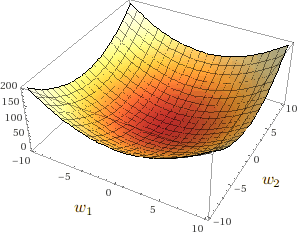
\includegraphics[height=150px,keepaspectratio]{descenso_gradiente_1.png}
  \caption{Representación de la superficie continua formada por $E$, con respecto a $w_1$ y $w_2$. Las zonas más oscuras representan un menor valor de $E$. Los ejes $w_1$ y $w_2$ representan los posibles valores para los pesos mientras que el eje vertical es el error correspondiente a dichos pesos.}
  \label{fig:descenso_gradiente}
\end{figure}

Supongamos que $\vec{w}^{\,} = (w_1, w_2)$, en la Figura \ref{fig:descenso_gradiente} podemos observar la superficie continua formada por $E$ y $\vec{w}^{\,}$. Dado que el objetivo es minimizar el error, se deben encontrar los valores de $w_1$ y $w_2$ que estén en la región más oscura de la superficie. 

Para encontrar los valores $w_i$ que minimizan $E$, hay que computar la derivada de $E$ respecto a cada componente de $\vec{w}^{\,}$ para obtener así el vector \textit{gradiente}:

\begin{equation}
\nabla E(\vec{w}^{\,}) = (\dfrac{\partial E}{\partial w_1}, \dfrac{\partial E}{\partial w_2}, ..., \dfrac{\partial E}{\partial w_n}).
\end{equation}
\newline
\noindent Este vector especifica la dirección en la cual $E$ tiene un máximo crecimiento, por lo tanto, para obtener la dirección en donde la función más decrece, utilizaremos el opuesto del gradiente, es decir $- \nabla E(\vec{w}^{\,})$. Luego, actualizamos los pesos de la siguiente manera:
\newpage
\begin{equation}
w_i \leftarrow w_i+ \Delta w_i,
\end{equation}

\noindent donde

\begin{equation}\label{eq:param_act}
\Delta w_i = - \eta \dfrac{\partial E}{\partial w_i},
\end{equation}
\newline
\noindent $\eta$ es la \textit{tasa de aprendizaje} (learning rate), la cual se encarga de parametrizar cuánto nos movemos en dirección al mínimo. 

La tasa de aprendizaje es un hiperparámetro de la red y suele ser un número pequeño (0.1, 0.001, etc). Este hiperparámetro es uno de los más importantes a ajustar. Si es grande, tenemos la ventaja de que el algoritmo converge más rápido a la solución, dado que se dan pasos más largos en cada iteración. Aún así, corremos el peligro de sobrepasar el mínimo global y por lo tanto no converger al mismo. Si es pequeño, podemos movernos con más confianza, pero corremos el peligro de quedarnos atascados en un punto de ensilladura además de hacer el proceso mucho más lento.
\newline

Volviendo a la Ecuación \ref{eq:funcion_error}, para calcular el gradiente, se debe efectuar la siguiente derivada para cada una de las componentes de $\vec{w}^{\,}$:

\begin{equation}
  \begin{array}{ll}
\dfrac{\partial E}{\partial w_i} = & \dfrac{\partial}{\partial w_i} \dfrac{1}{2}\sum_{d \in D}{}{(t_d - o_d)^2} \\
~~~~~~= & \sum_{d \in D}{}{(t_d - o_d)}\dfrac{\partial}{\partial w_i}(t_d - \vec{w}^{\,}.\vec{x_d}^{\,})	 \\
~~~~~~= & \sum_{d \in D}{}{(t_d - o_d)}(-x_{id}),
  \end{array}
\end{equation}
\newline
\noindent donde $x_{id}$ es el componente $i$ del ejemplo de entrenamiento $d$. Luego, substituyendo en la Ecuación \ref{eq:param_act} se obtiene

\begin{equation}\label{eq:param_act_concreto}
\Delta w_i = - \eta \sum_{d \in D}{}{(t_d - o_d)}(-x_{id}).
\end{equation}

Finalmente, el proceso se reduce a repetir el cálculo de la Ecuación \ref{eq:param_act_concreto} y actualizar los pesos hasta que se cumpla alguna condición de terminación. 

\subsubsection{Descenso por el gradiente estocástico}

Existe un problema importante con el algoritmo anterior que es el de la velocidad de convergencia. Como se puede ver en la Ecuación \ref{eq:param_act_concreto}, la actualización de pesos se hace después de realizar la suma sobre todos los ejemplos de entrenamiento de $D$.

En el caso del descenso por el gradiente estocástico \cite{Mitchell97a}, la actualización de pesos se hace en forma incremental, calculando el error para cada uno de los ejemplos individualmente. El algoritmo resultante se pude ver en Algoritmo \ref{alg:gradiente_est}.

\begin{algorithm}
\caption{Descenso por el gradiente estocástico}
\begin{algorithmic}[1]
	\label{alg:gradiente_est}
  \STATE Inicializar cada $w_i$ con algún número aleatorio pequeño.
  \STATE Hasta que una condición de terminación se cumpla, hacer:
  \begin{itemize}
	\itemsep0em 
  	\item Inicializar cada $\Delta w_i$ en cero.
  	\item Por cada $\langle \vec{x}^{\,}, t \rangle$ en los ejemplos de entrenamiento, hacer:
  	\begin{itemize}
		\itemsep0em 
  		\item Utilizar $\vec{x}^{\,}$ como entrada para obtener la salida $o$
  		\item Por cada peso $w_i$ hacer $w_i \leftarrow w_i+ \Delta w_i$
  	\end{itemize}
  \end{itemize}
\end{algorithmic}
\end{algorithm}

Esta versión es mucho más rápida que la versión convencional del descenso por el gradiente. Un ajuste que se le puede hacer al algoritmo es utilizar minibatches. En lugar de recorrer cada uno de los ejemplos de entrenamiento para luego actualizar los pesos, lo que se hace es dividir el conjunto en subconjuntos de tamaño $k$ y actualizar los pesos por cada subconjunto procesado. La ventaja de utilizar minibatches es que es trivialmente paralelizable, lo que nos permite aprovechar mejor las GPUs.

El método conocido como \textit{backpropagation} consiste en hacer el descenso por el gradiente calculando de manera eficiente las derivadas de cada parámetro. Las neuronas que son alcanzadas cuando se propaga hacia atrás el error no reciben el mismo de forma completa, sino que reciben una fracción proporcional a la contribución que tuvieron con respecto al error obtenido. Cuando se realiza la actualización de pesos con el descenso por el gradiente se hace teniendo en cuenta esta contribución.

%%\subsubsection{Backpropagation}

%%Es un algoritmo que hace uso del desceso por el gradiente estocástico para recalcular los pesos de una red neuronal con un número de neuronas arbitrario donde las mismas tienen una función de activación derivable. 
%%El primer paso, conocido como \textit{propagación hacia adelante} (forward pass) es obtener una salida a desde de un ejemplo de entrenamiento $x_i$ y a partir de esta calcular el error. Una vez obtenido el error, el mismo se \textit{propaga hacia atrás} (backward pass), desde las neuronas de salida hacia las capas ocultas.

%%Las neuronas que son alcanzadas en el backward pass no reciben el error de forma completa, sino que reciben una fracción proporcional a la contribución que tuvieron con respecto al error obtenido. Cuando se realiza la actualización de pesos con el descenso por el gradiente se hace teniendo en cuenta esta contribución.

%% Se hace el descenso por el gradiente comun, pero en este caso se multiplica la contribucion de la neurona por la actualizacion del peso, para corregir el peso en proporcion la contribucion de su error.

\subsection{Optimización del aprendizaje}

La forma de entrenamiento presentada hasta el momento tiene varias deficiencias. Puede suceder que durante el aprendizaje el algoritmo quede atrapado en un punto de ensilladura o que algunos pesos crezcan de forma desmedida afectando la capacidad de generalización. A continuación, se presentan algunas técnicas de optimización para tratar estos problemas.

\subsubsection{Preparación de los datos para el entrenamiento}

Antes de comenzar con el entrenamiento se deben preparar los datos de entrada \cite{curso_stanford}. Una primer medida a tomar es \textit{sustraer la media} (Figura \ref{fig:prepocesamiento_datos}, segunda columna) de cada característica individual de los datos. Esto se puede interpretar geométricamente como centrar los datos lo más cerca del origen que se pueda en cada dimensión. Por ejemplo, para imágenes, la sustracción de la media debe hacerse para cada canal de color individualmente.

Otra técnica de preprocesamiento muy utilizada es \textit{normalizar} los datos (Figura \ref{fig:prepocesamiento_datos}, tercer columna). La normalización consiste en llevar a todas las dimensiones que pueda tener la entrada a la misma escala. Una forma de hacerlo es dividir cada dimensión por su desviación estándar, luego de haber sido centrada en el origen. Otra forma de normalización es llevar el mínimo y el máximo de cada dimensión a $-1$ y $1$ respectivamente. Sólo tiene sentido aplicar la normalización cuando las diferentes características tienen diferente escala entre sí, pero son igualmente importantes para el problema.

\begin{figure}[H]
\centering
 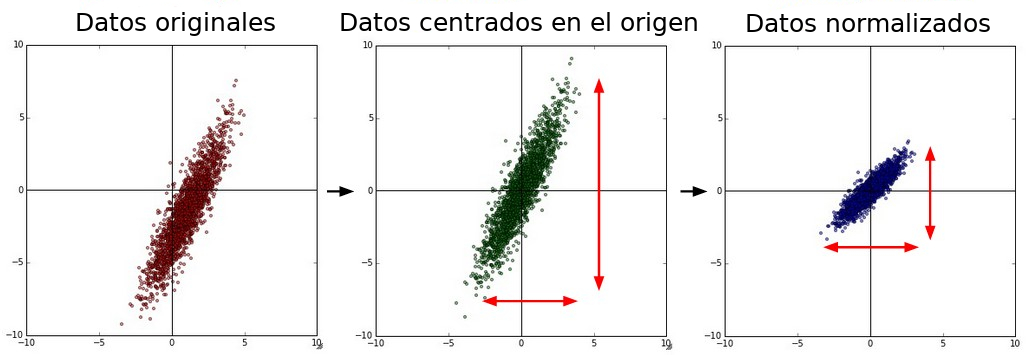
\includegraphics[width=\linewidth]{prepro1.jpeg}
  \caption[Preprocesamiento de datos]{Preprocesamiento de datos \protect\footnotemark}
  \label{fig:prepocesamiento_datos}
\end{figure}
\footnotetext{Imagen tomada de \url{http://cs231n.github.io/neural-networks-2/.}}

Algo importante a destacar es que cualquier preprocesamiento estadístico sólo debe ser computado en los datos de  entrenamiento y luego aplicado a los datos de validación y/o test. Por ejemplo, computar la sustracción de la media en todo un dataset y luego dividirlo en entrenamiento, validación y test es un error. En lugar de eso, la media debe ser computada sólo sobre los datos de entrenamiento y luego sustraída de forma equivalente en los tres conjuntos.

\subsubsection{Batch normalization}

Es una técnica que permite aumentar la estabilidad y la velocidad de entrenamiento de una red. En lugar de normalizar sólo los datos de entrada, también se normalizan las entradas de las capas ocultas de la red por cada minibatch. Esta técnica ayuda a mitigar el problema del \textit{internal covariance shift}. 

Internal covariance shift es el cambio en la distribución de las activaciones de una capa a raíz del cambio de los parámetros de la capa anterior. En otras palabras, cuando los parámetros de una capa cambian, también lo hace la distribución de entradas de las capas subsiguientes. A continuación se dará un ejemplo sencillo de covariance shift simple, pero que es esperable que el mismo genere cambios en las representaciones internas de la red. Supongamos que tenemos una red neuronal para detectar gatos en una imagen. La red está entrenada solamente con imágenes de gatos negros. Si intentamos utilizar esta red para detectar gatos de colores en lugar de negros la red va a fallar en la mayoría de los casos. Es decir, si el algoritmo aprendió un mapeo de $X$ a $Y$, y la distribución de $X$ cambia, entonces es muy probable que tengamos que re-entrenar la red.

Batch normalization normaliza las activaciones de la capa anterior sustrayendo la media del minibatch y dividiendo el mismo por su desviación estándar. Luego de esta normalización, los pesos de la capa siguiente no son óptimos para los valores de entrada dada la conversión, por lo que el descenso por el gradiente estocástico ``deshace'' la normalización si es una forma de minimizar la función de costo. Por este motivo, se agregan dos parámetros entrenables, por lo que la salida normalizada se multiplica por una ``desviación estándar'' ($\gamma$) y se le suma una ``media'' ($\beta$). Estos parámetros se conocen como parámetros de desnormalización y tienen el propósito de permitirle al descenso por el gradiente desnormalizar los datos a través de ellos en lugar de cambiar todos los pesos de la red.
Dado que batch normalization previene que las activaciones tengan valores muy altos o muy bajos, se puede utilizar un learning rate más alto, lo cual tiene como consecuencia un aumento en la velocidad de entrenamiento. 


\subsubsection{Weight decay}

Cuando existen pesos muy grandes, la red es mucho más sensible al ruido de los datos de entrada, por lo tanto, cuando éste es propagado por una red con pesos grandes, produce una salida muy distinta en relación a una red con pesos más pequeños y balanceados. Los pesos grandes suelen estar correlacionados con características particulares del conjunto de entrenamiento por lo que afecta a la generalización.

\textit{Weight Decay} \cite{Mitchell97a} es una técnica de regularización que se utiliza para prevenir el sobreajuste. Consiste en decrementar cada uno los pesos por un factor muy pequeño en cada iteración. Esto previene que los pesos crezcan desmedidamente. Para medir qué tan grandes son los pesos, se usan términos de regularización \cite{curso_stanford}. Los más utilizados son:
\newpage
\begin{itemize}
\item L1: Se implementa penalizando el valor absoluto de los pesos. Esto es, por cada peso $w_i$ computamos el término $\lambda |w_{i}|$, donde $\lambda$ es la fuerza de la regularización. 
\item L2: Se implementa penalizando el cuadrado de los pesos. Esto es, por cada peso $w_i$ computamos el término $\frac{1}{2} \lambda w_{i}^{2}$, donde $\lambda$ es la fuerza de la regularización. Esta regularización penaliza los vectores con pesos desbalanceados (con mucho más peso en algunas componentes que en otras), prefiriendo vectores más difusos.
\end{itemize}

Dado que es matemáticamente equivalente, en lugar de decrementar cada uno de los pesos por separado, se cambia la definición de la función de costo, incluyendo un término de penalización con la suma de todos los pesos de la red. Luego, la función nos queda reformulada de la siguiente manera:

\begin{equation}
L1: \hat E(\vec{w}^{\,}) = E(\vec{w}^{\,}) + \lambda\sum_{i,j}^{}{|w_{i,j}|},
\end{equation}

\begin{equation}
L2: \hat E(\vec{w}^{\,}) = E(\vec{w}^{\,}) + \frac{\lambda}{2}\sum_{i,j}^{}{w_{i,j}^{2}}.
\end{equation}

\subsubsection{Dropout}

Es otra técnica de regularización propuesta por Srivastava, et al. \cite{dropout_paper}. El término \textit{dropout} (del inglés drop - tirar) refiere a ``tirar'' neuronas (tanto de la capa oculta como de la capa de entrada) durante el entrenamiento. En otras palabras, se remueven temporalmente de la red junto con sus conexiones de entrada y de salida.

La elección de qué neuronas tirar es aleatoria. En el caso más simple, cada neurona es conservada con una probabilidad $p$ independientemente de las demás neuronas. El dropout es utilizado solamente en el entrenamiento, en todas las demás fases se usa la red completamente conectada.

\begin{figure}[H]
\centering
 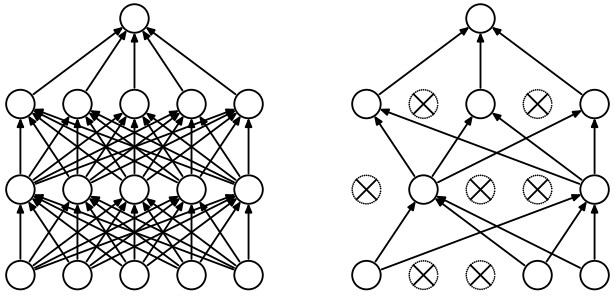
\includegraphics[width=\linewidth]{dropout.jpeg}
  \caption[A la izquierda, una red completamente conectada. A la derecha, la misma red luego de aplicar dropout.]{A la izquierda, una red completamente conectada. A la derecha, la misma red luego de aplicar dropout. \protect\footnotemark}
  \label{fig:dropout}
\end{figure}
\footnotetext{Imagen tomada del paper original \cite{dropout_paper}.}

%% https://machinelearningmastery.com/dropout-regularization-deep-learning-models-keras/ -> de aca sale la ultima oracion

Aplicar dropout significa entrenar redes más ``delgadas'', siendo éstas un subconjunto de la red original. Gracias al entrenamiento con dropout, la red se vuelve menos sensible a pesos específicos, mejorando así la generalización.

\subsubsection{Momentum}

La superficie de error a explorar puede ser muy compleja y contener varios puntos de ensilladura. El \textit{momentum} \cite{Mitchell97a} es un hiperparámetro utilizado para evitar quedarnos atrapados en estos puntos de ensilladura. Se introduce modificando la regla de actualización de pesos, haciéndola depender parcialmente de lo que ocurrió en la actualización de pesos de la iteración anterior:

\begin{equation}
\Delta w_i(n) = \eta (t - o) x_i + \alpha \Delta w_i (n - 1).
\end{equation}


\noindent Donde $\Delta w_i(n)$ es la actualización de pesos hecha en la iteración $n$ y $0 \leq \alpha < 1$ es el hiperparámetro llamado \textit{momentum}.

De forma más intuitiva, consideremos que la trayectoria hecha por el descenso por el gradiente es análoga a una pelota (sin momentum) bajando por la superficie de error. El efecto de $\alpha$ es el de agregar \textit{momentum} para que la pelota siga girando en la misma dirección de una iteración a otra. De este modo, no quedaría atrapada dentro de pequeños pozos, porque la inercia la hará sobrepasarlos.


\subsubsection{Adam}

Adam \cite{adam_paper} \cite{deep_learning_book} es un método de optimización que puede ser utilizado en reemplazo del descenso por el gradiente tradicional para actualizar los pesos de la red. En lugar de tener solamente un learning rate para toda la red, Adam mantiene uno por cada peso, que se van actualizando por separado a medida que el entrenamiento transcurre. El método combina las ventajas de otras dos extensiones del descenso por el gradiente:

\begin{itemize}
\item{\textbf{Adaptive Gradient Algorithm} (AdaGrad) \cite{deep_learning_book}: Este algoritmo va adaptando los learning rates de cada peso escalándolos de forma inversamente proporcional a la raíz cuadrada de la suma de todos sus valores históricos al cuadrado. Los parámetros con una mayor derivada parcial con respecto a la pérdida tienen un decremento rápido de su learning rate mientras que los parámetros con una menor derivada parcial tienen un decremento relativamente pequeño de su learning rate.}

\item{\textbf{Root Mean Square Propagation} (RMSProp) \cite{deep_learning_book}}: Es una optimización de AdaGrad que cambia la acumulación valores históricos del gradiente por una media móvil exponencial\footnote{La \textbf{media móvil exponencial} es una media móvil ponderada exponencialmente. Se trata de la media aritmética de los $n$ valores anteriores con factores de ponderación que decrecen exponencialmente. La ponderación para cada punto de datos más antiguos decrece exponencialmente, nunca llegando a cero. Da mayor importancia a los datos más recientes.}. AdaGrad está diseñado para converger rápido cuando es aplicado a una función convexa. Cuando no es aplicado sobre este tipo de función para entrenar una red neuronal, la trayectoria de aprendizaje puede pasar por diferentes estructuras y eventualmente llegar a una región convexa. Dado que AdaGrad decrece el learning rate teniendo en cuenta todo el historial, puede que éste sea demasiado pequeño al momento de arribar a dicha región. Al utilizar la media móvil exponencial, RMSProp descarta el histórico distante para poder converger rápido al encontrar un área convexa, como si fuese una instancia de AdaGrad inicializada en sobre este tipo de zona. Al utilizar RMSProp introducimos un hiperparámetro $\rho$ para controlar la longitud de escala de la media exponencial.

\end{itemize}

\noindent Adam no sólo usa la media móvil para adaptar los learning rates de cada parámetro sino que también utiliza la varianza móvil. Los hiperparámetros existentes para este método son $\beta 1$, el cual controla la tasa de decaimiento para la media móvil (recomendado en $0.9$) y $\beta 2$, el cual controla la tasa de decaimiento para la varianza móvil (recomendado en $0.999$).

\section{Deep Learning}

Una gran dificultad que enfrenta la inteligencia artificial en problemas del mundo real es que los datos que observamos son afectados por muchos factores de variabilidad. Por ejemplo, los píxeles de una imagen de un auto rojo pueden estar más cerca de ser negros que rojos si la foto fue tomada de noche. La silueta del auto depende del ángulo de visión. 

\textit{Deep learning} \cite{deep_learning_book} resuelve este problema introduciendo representaciones que son expresadas en términos de otras representaciones más simples. En otras palabras, permite construir conceptos complejos a partir de conceptos más simples. La Figura \ref{fig:deep_learning_ex} muestra cómo un sistema de deep learning basado en redes neuronales puede representar el concepto de la imagen de una persona combinando conceptos más simples, como los bordes y contornos, éstos últimos definidos a partir de bordes.

\begin{figure}[h]
\centering
 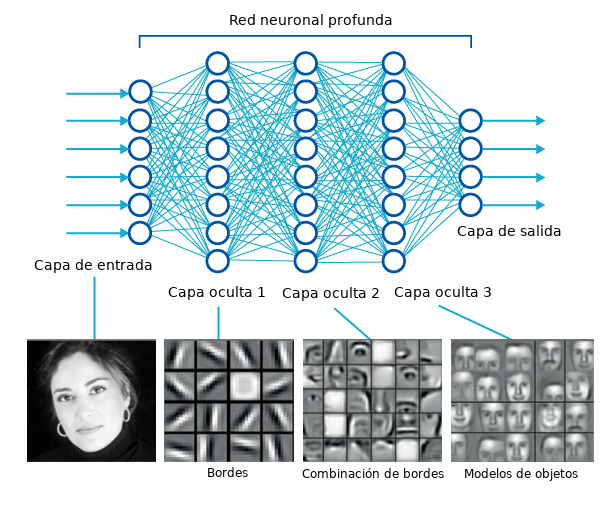
\includegraphics[width=\linewidth]{deep_learning_ex.jpg}
   \caption[Ilustración de un modelo de deep learning basado en redes neuronales. En la capa de entrada tenemos la imagen a reconocer. La primer capa oculta se encarga de la detección de bordes. La segunda capa oculta se encarga de la detección de contornos (definidos a partir de bordes). La tercer capa se encarga de la detección de objetos (definidos a partir de contornos).]{Ilustración de un modelo de deep learning basado en redes neuronales. En la capa de entrada tenemos la imagen a reconocer. La primer capa oculta se encarga de la detección de bordes. La segunda capa oculta se encarga de la detección de contornos (definidos a partir de bordes). La tercer capa se encarga de la detección de objetos (definidos a partir de contornos). \protect\footnotemark}
  \label{fig:deep_learning_ex}
\end{figure}

\footnotetext{Imagen tomada de \url{https://www.saagie.com/fr/blog/object-detection-part1}.}

Existen dos formas de medir la profundidad de un modelo. La primera está basada en la cantidad de instrucciones secuenciales que deben ser ejecutadas para evaluar la arquitectura. Podemos pensar esta perspectiva como la longitud del camino más largo a través de un diagrama de flujo que describe cómo computar cada una de las salidas del modelo dadas sus entradas. La segunda, utilizada por modelos probabilísticos profundos, toma como profundidad del modelo la profundidad del grafo que describe cómo los conceptos se relacionan entre sí en lugar de la profundidad del grafo computacional.

Dado que no siempre es claro cuál de estos dos enfoques es el más relevante, no existe un valor único que represente la profundidad de una arquitectura ni tampoco hay un consenso de cuánta profundidad debe tener un modelo para poder ser clasificado como  ``profundo''. Sin embargo, uno puede decir con seguridad que deep learning es el estudio de modelos que contienen una gran cantidad de composición de conceptos aprendidos en comparación con los modelos tradicionales de machine learning \cite{deep_learning_book}.

\subsection{Redes generativas adversarias}

Las redes generativas adversarias (GANs) \cite{goodfellow_generative_2014} \cite{gan_explanation_web} son un conjunto de redes ideadas para entrenar modelos generativos a partir de la competencia entre un modelo generativo y un modelo discriminativo.  Una GAN está compuesta por dos redes neuronales, un generador $G$ que a partir de ruido como entrada genera una imagen, y un discriminador $D$ que tiene como objetivo clasificar las imágenes del dataset como reales y las generadas por $G$ como falsas. El discriminador se entrena de la manera usual para un problema de clasificación binaria mientras que el generador, en cambio, se entrena para engañar al discriminador.

El generador se define como una función $G(z)$, que toma una entrada $z$ (normalmente un vector de ruido) de una distribución de probabilidades simple $\rho_z(z)$ e intenta mapear dicha entrada a un $x$ perteneciente a $\rho_{data}(x)$, que es la distribución de los datos reales. El discriminador se define como una función $D(x)$, que toma una entrada $x$ de la unión entre la distribución $\rho_{data}(x)$ y la distribución de imágenes falsas y tiene como salida un número en el intervalo $[0, 1]$, indicando la probabilidad de que dicha entrada $x$ sea falsa (generada por $G$) o verdadera (proveniente de los datos reales). Ambas son funciones diferenciables representadas por una red neuronal.

El generador es entrenado para intentar engañar al discriminador de forma tal que éste clasifique a una entrada generada por sí mismo como verdadera. El discriminador es entrenado para distinguir las muestras reales de las falsas, siendo éstas últimas cada vez más convincentes, resultado del entrenamiento del generador. Más formalmente, $G$ y $D$ juegan un juego de dos jugadores que puede ser modelado con minimax a través de una función de valor $V(G, D)$ donde:

\begin{equation}\label{eq:minimax_1}
V(G, D) = \mathds{E}_{x\sim\rho_{data}(x)}[log(D(x))] + \mathds{E}_{x\sim\rho_{z}(z)}[log(1 - D(G(z)))],
\end{equation}

\begin{equation}\label{eq:minimax_2}
\min_{G}\max_{D} V(G, D).
\end{equation}

~\\
En la Ecuación \ref{eq:minimax_1}, el primer término es el logaritmo de la probabilidad de que el discriminador $D$ prediga una muestra obtenida de $\rho_{data}(x)$ (distribución de datos reales) como verdadera. El discriminador intenta maximizar esto a 1. El segundo término es el logaritmo de la probabilidad de que el discriminador $D$ prediga una muestra de la distribución $\rho_{z}(z)$ pasadas a través del generador $G$ como falsa. El discriminador intenta maximizar esto a 0. Es decir, el discriminador está intentado maximizar la función $V(G, D)$ (Ecuación \ref{eq:minimax_2}).

Por otro lado, la tarea del generador es exactamente la opuesta, dado que intenta minimizar la función $V(G, D)$ (Ecuación \ref{eq:minimax_2}) para que la diferencia entre las muestras falsas y las verdaderas sean mínimas.

\subsubsection{Entrenando una GAN}

El entrenamiento de una GAN se puede dividir en dos grandes fases. Primero se entrena el discriminador congelando\footnote{Hacer sólo el forward pass, omitiendo la actualización de pesos.} el generador. Una vez terminado el entrenamiento del discriminador se repite el proceso, pero esta vez congelando el discriminador y entrenando el generador. El procedimiento se repite hasta que se cumpla alguna condición de terminación. Más detalladamente, los pasos para entrenar una GAN son los siguientes:

\begin{enumerate}
\item Definir la arquitectura de la GAN: Dependiendo del problema pueden ser las dos redes convolucionales, perceptrones de múltiples capas u otro tipo de redes.
\item Entrenar el discriminador en datos reales por \textit{n} épocas: Tomar los datos reales de los cuales queremos generar los datos falsos y entrenar al discriminador para que correctamente los prediga como verdaderos.
\item Generar datos falsos con el generador y entrenar el discriminador con éstos: Tomar los datos generados y dejar que el discriminador los prediga correctamente como falsos.
\item Entrenar al generador con la salida del discriminador: Con la salida de los puntos 2 y 3 entrenamos el generador para que intente engañar al discriminador.
Repetir del paso 2 al 4 hasta que se cumpla alguna condición de terminación.
\end{enumerate}

\subsection{Wasserstein GANs}

Normalmente en los modelos generativos se intenta aprender una distribución de probabilidades \cite{wgan_web}. Esto comúnmente se hace definiendo una familia de funciones de densidad de probabilidad $(P_{\theta})_{\theta\in\mathbb{R}^d}$ y encontrando la que maximiza la verosimilitud o likelihood con los datos reales.

Si tenemos que $\mathbb{P}_{r}$ es la distribución de los datos reales y $\mathbb{P}_{\theta}$ es la distribución que queremos aproximar a $\mathbb{P}_{r}$ con una función de densidad $P_{\theta}$, este problema se puede resolver minimizando la divergencia de Kullback-Leibler\footnotemark $KL(\mathbb{P}_{r}||\mathbb{P}_{\theta})$ 

\footnotetext{La divergencia de Kullback-Leibler (KL) es una medida no simétrica de la similitud o diferencia entre dos funciones de distribución de probabilidad P y Q.}

Existen casos en los que $P_{\theta}$ tiene un soporte de baja dimensión, lo que trae como consecuencia que KL no exista o sea infinita. Para remediar esta situación se agrega un término de ruido a la distribución. El ruido agregado afecta de forma negativa al modelo, pero es necesario para hacer que esta forma de resolver el problema funcione. En el caso de las imágenes, por ejemplo, inyectar ruido en el modelo hace que las imágenes salgan con menos definición.

Las Wasserstein GANs \cite{wgan_paper} toman otro enfoque para resolver este problema. En lugar de estimar la densidad de $\mathbb{P}_{r}$, que puede no existir, se define una variable aleatoria $Z$ (normalmente de una distribución gaussiana o uniforme) con una distribución $\rho(z)$ y se pasa a través de una función  $g_{\theta}$ (generalmente es una red neuronal de algún tipo, en nuestro caso la red generadora de una GAN) que directamente genere ejemplos siguiendo una cierta distribución $\mathbb{P}_{\theta}$. Variando $\theta$, se puede ir cambiando la distribución y hacerla cada vez más cercana a $\mathbb{P}_{r}$. En otras palabras buscamos que $\mathbb{P}_{r} = g_{\theta}(Z)$.

Para entrenar $g_{\theta}$ debemos tener una forma de medir distancia entre las distribuciones. Es decir, necesitamos una función $d(\mathbb{P}_{\theta}, \mathbb{P}_{r})$ que nos diga cuán lejos está una distribución de la otra. Si tomamos dicha función como la función de costo, minimizar $d(\mathbb{P}_{\theta}, \mathbb{P}_{r})$ con respecto a $\theta$, hace que $\mathbb{P}_{\theta}$ se acerque a $\mathbb{P}_{r}$.


\subsubsection{Distancia de Wasserstein o Earth Mover Distance}

La función de distancia que vamos a utilizar es la EMD (Earth Mover Distance) \cite{earth_move_distance}. Las distribuciones de probabilidad están definidas por cuanta ``masa'' o peso le ponen a los puntos. Supongamos que empezamos con una distribución $\mathbb{P}_{\theta}$, y queremos ir moviendo masa para transformarla en $\mathbb{P}_{r}$. Mover una masa $m$ una distancia $d$ cuesta un esfuerzo de $m * d$. La EMD es el mínimo esfuerzo que debemos hacer. Si imaginamos que las distribuciones son diferentes montículos de una determinada cantidad de tierra, entonces la EMD es la cantidad total de trabajo que se necesita para convertir un montículo en el otro. La Figura \ref{fig:emd} muestra la forma óptima de convertir una distribución en otra transportando su masa.


\begin{figure}[h]
\centering
 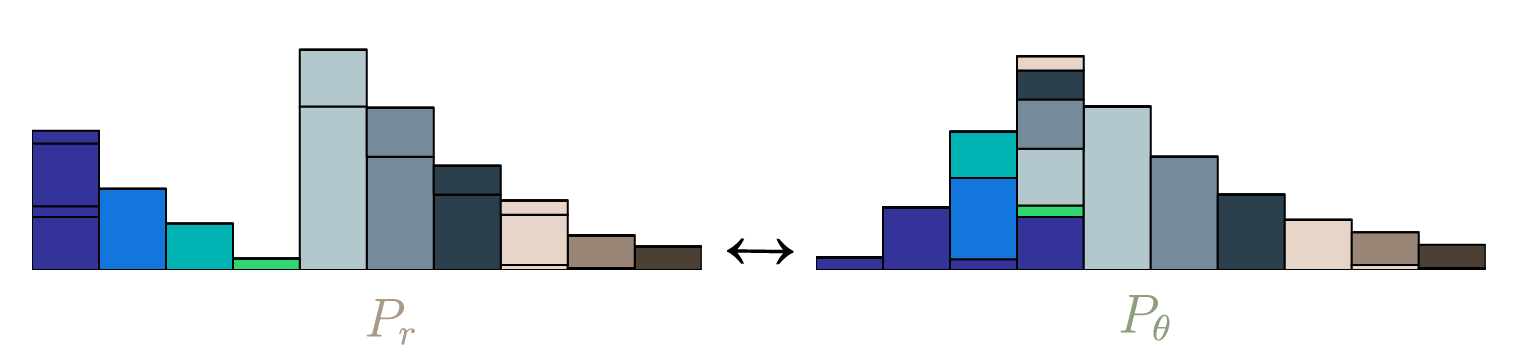
\includegraphics[width=\linewidth]{earth_move.png}
   \caption[Movimientos óptimos de transporte de masa entre $\mathbb{P}_{r}$ y $\mathbb{P}_{\theta}$]{Movimientos óptimos de transporte de masa entre $\mathbb{P}_{r}$ y $\mathbb{P}_{\theta}$ \protect\footnotemark}
  \label{fig:emd}
\end{figure}

\footnotetext{Imagen tomada de \url{https://vincentherrmann.github.io/blog/wasserstein/}.}
\newpage
	Dado que hay infinitas formas de mover la masa de una distribución a otra, encontrar el óptimo es un problema de optimización lineal. En lugar de utilizar la distancia se usa una aproximación a la misma.
	
%%Para la aproximación se utiliza una familia de funciones llamadas K-Lipschitz. Una función $f:X \rightarrow Y$ es K-Lipschitz si, dados dos funciones de distancia $d_{x}$ y $d_{y}$ en espacios $X$ e $Y$ se cumple que

%\begin{equation}
% d_{y}(f(x), f(y))  \leq  Kd_{x}(x, y).
%\end{equation}

%\noindent para todo $x, y \in X$, $K \in \mathbb{R}$.

%Con esto definimos una familia de funciones K-Lipschitz para algún K, $\{ f_{w} \}$, $w \in W$, donde $W$ es el conjunto de todos los pesos posibles. 




%	Gracias a estas funciones, tenemos una forma de aproximar la EMD. No vamos a ahondar en los detalles matemáticos, pero para dar un panorama: Supongamos que tenemos una familia de funciones {fw} w W, donde Wes el conjunto de todos los pesos posibles. También tenemos que estas funciones son todas K-Lipschitz para algún K. No hace falta conocer el K, con saber que existe es suficiente.


\subsubsection{Entrenamiento de una WGAN}

Nuestro objetivo es entrenar $\mathbb{P}_{\theta} = g_{\theta}(Z)$, para que se acerque a $\mathbb{P}_{r}$. El proceso de entrenamiento para el discriminador es:\\

\noindent Sea $W(\mathbb{P}_{r}, \mathbb{P}_{\theta})$ la EMD entre $\mathbb{P}_{r}$ y $\mathbb{P}_{\theta}$:

\begin{itemize}
\item Para un $\theta$ fijo, computamos la aproximación de $W(\mathbb{P}_{r}, \mathbb{P}_{\theta})$.
\item Una vez obtenida dicha aproximación, computamos el gradiente $\nabla_{\theta} W(\mathbb{P}_{r}, \mathbb{P}_{\theta})$ utilizando varios ejemplos de $z \sim Z$
\item Actualizar $\theta$ y repetir.
\end{itemize}

\noindent Para poder calcular las aproximaciones de $W(\mathbb{P}_{r}, \mathbb{P}_{\theta})$ debemos limitar los pesos a un intervalo $[-c, c]$, $c \in \mathbb{R}$.


\subsubsection{Contraste con las GANs}

En las GANs el discriminador siempre tiene como salida un valor en el intervalo $[0, 1]$ representando una probabilidad. En WGANs, no necesariamente se obtiene como salida un valor del intervalo anteriormente nombrado, es por eso que en lugar de llamarlo discriminador, lo llamamos crítico, ya que no está explícitamente intentando clasificar una entrada como verdadera o falsa. En lugar de esto, mide qué tan distante está lo que generó $g_{\theta}$ de lo real. Por ejemplo, supongamos que tenemos un crítico de arte. Le damos un Picasso falso y éste nos responde “está dos veces mejor que el falso Picasso anterior y todavía se ve 5 veces peor que el original”. De esta manera, el crítico puede enseñar de una mejor forma al generador.
\newpage
Otra diferencia es que en las GANs nunca se entrena el discriminador hasta la convergencia. Lo que usualmente se hace es ir alternando las actualizaciones de los gradientes entre el discriminador y el generador para obtener una actualización de pesos que tenga sentido. En WGANs se puede entrenar el crítico hasta la convergencia, para estimar una mejor EMD, lo cual deriva en un gradiente $\nabla_{\theta} W(\mathbb{P}_{r}, \mathbb{P}_{\theta})$ más exacto y por lo tanto en una mejor actualización de los pesos.

\subsection{Redes Convolucionales}

Las redes neuronales convolucionales \cite{curso_stanford} \cite{web_conv} son muy similares a las redes vistas hasta el momento: están construidas a partir de neuronas artificiales con pesos y biases que se pueden aprender. Cada neurona recibe algunas entradas, realiza un producto vectorial y opcionalmente se aplica una función de activación. La diferencia radica en que las redes convolucionales asumen explícitamente que las entradas son imágenes, lo que permite codificar ciertas propiedades dentro de la arquitectura con el objetivo de hacer la función de evaluación más eficiente y reducir el número de parámetros en la red.

Una imagen está formada por una matriz de píxeles, donde cada píxel está definido por una tripleta que contiene tres números enteros en el rango $[0, 255]$, siendo la primer componente el color rojo, la segunda el color verde y la tercera el color azul. Los valores cercanos a 0 representan la ausencia de luz mientras que los cercanos a 255 la presencia de luz de un determinado color. Por ejemplo, un píxel con el valor $(255, 0, 0)$ es un píxel completamente rojo. Alternativamente, una imagen se puede pensar como tres matrices bidimensionales compuestas por números en el rango $[0, 255]$ donde cada matriz representa una capa de color elemental (Figura \ref{fig:img_capas_rgb}). Estas capas son conocidas como canales.

\begin{figure}[h]
\centering
 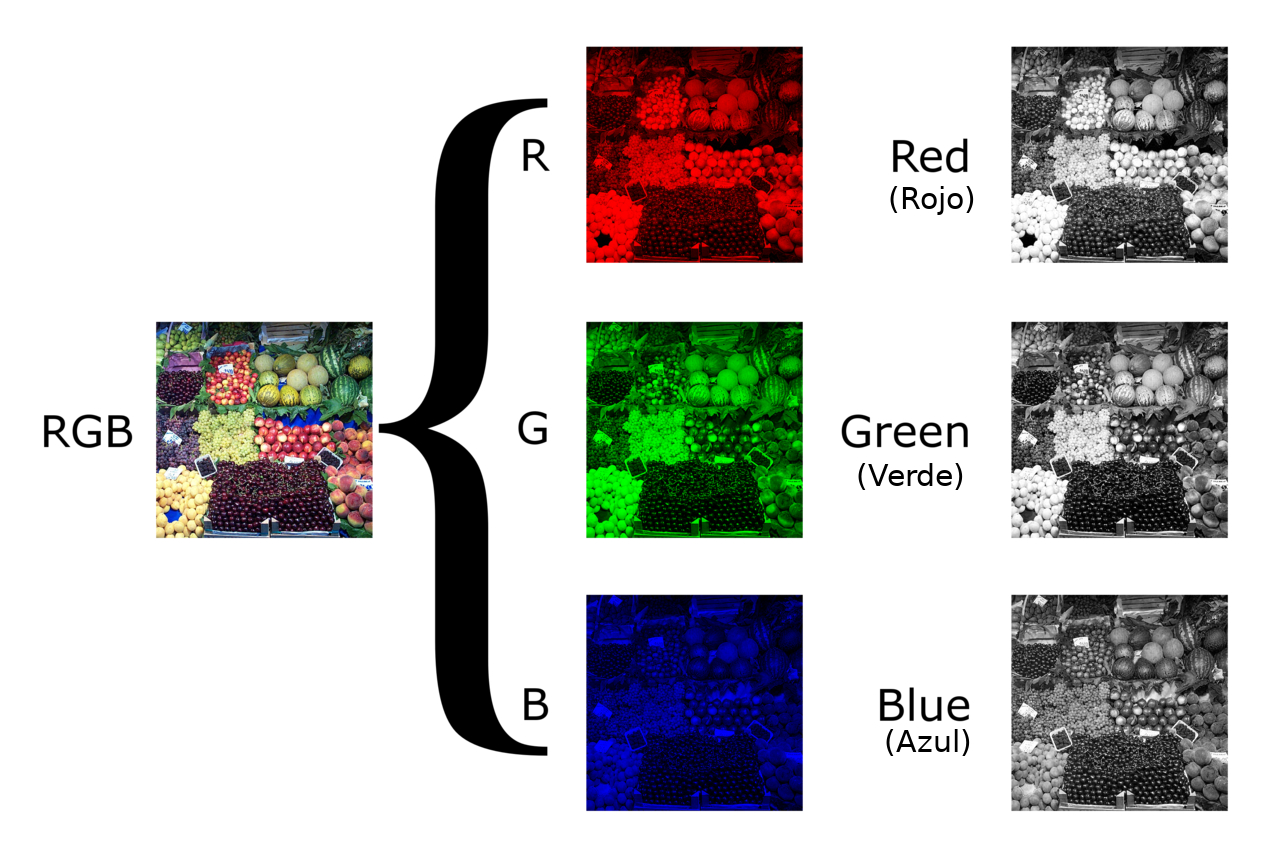
\includegraphics[width=\linewidth]{rgb_imagen.jpg}
   \caption[Descomposición de una imagen en sus tres canales elementales.]{Descomposición de una imagen en sus tres canales elementales. \protect\footnotemark}
  \label{fig:img_capas_rgb}
\end{figure}
\footnotetext{Imagen tomada de \url{https://en.wikipedia.org/wiki/Grayscale}.}


Las redes neuronales convencionales no escalan bien con imágenes. Por ejemplo, en CIFAR10 \cite{cifar10}, las imágenes tienen un tamaño de $32*32*3$ (32 de ancho, 32 de alto y 3 canales de color), por lo que una capa oculta completamente conectada tendría $32*32*3=3072$ pesos por cada neurona. 
\newpage
A diferencia de las redes convencionales, las capas de una red convolucional están organizadas en tres dimensiones (Figura \ref{fig:red_conv}): ancho, alto y profundidad (con profundidad nos referimos a una medida de volumen de activaciones, y no a la profundidad de la red). Por ejemplo, si tomamos como entrada una imagen de CIFAR10, la capa de entrada contiene un volumen de activación de $32*32*3$ siendo el ancho, alto y profundidad (en este caso cada canal de la imagen) respectivamente. 

\begin{figure}[h]
\centering
 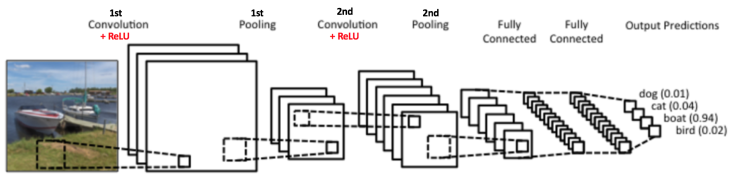
\includegraphics[width=\linewidth]{convnet.png}
   \caption[Representación de una red convolucional completa con todas sus capas.]{Representación de una red convolucional completa con todas sus capas. \protect\footnotemark}
  \label{fig:red_conv}
\end{figure}

\footnotetext{Imagen tomada de \cite{web_conv}.}

A continuación veremos las capas que se utilizan para construir una red convolucional.

\subsubsection{Capa de convolución}

El propósito de la capa de convolución es extraer características de la imagen de entrada. Los parámetros de la misma consisten en un conjunto de filtros que pueden aprenderse. Cada filtro es una matriz pequeña multidimensional. Por ejemplo, un filtro en la primera capa convolucional de una red puede tener un tamaño de $5*5*3$ (5 píxeles de ancho, 5 de alto y 3 de profundidad correspondiente a los canales de la imagen). En el forward pass, cada filtro se pasa a lo largo y a lo ancho de la imagen de entrada (Figura \ref{fig:convolution}) donde se computa el producto escalar entre el filtro y la entrada produciendo una matriz bidimensional de activaciones llamada llamada \textit{feature map} o \textit{activation map}.

\begin{figure}[h]
\centering
 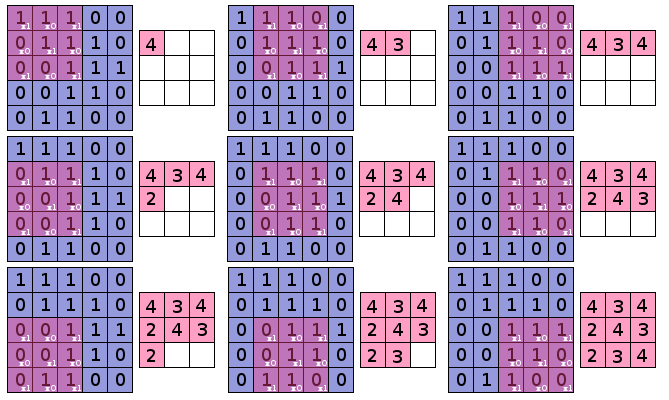
\includegraphics[width=\linewidth]{convolucion.png}
   \caption{Ejemplo simplificado de una convolución. La matriz color azul es una representación simplificada de una imagen a la que se le aplica la convolución. Sobre ella se va pasando el filtro, representado por la matriz color violeta. Como resultado obtenemos la matriz color rosa, llamada \textit{feature map} o \textit{activation map}.}
  \label{fig:convolution}
\end{figure}
\enlargethispage{0.6in}
Es importante notar que los filtros funcionan como detectores de características de la entrada a la que se los aplica. A medida que se entrena, la red va aprendiendo filtros que se activan cuando detectan algún tipo de característica visual como un borde o una mancha de un determinado color. Mientras vamos avanzando en las capas, las más internas pueden detectar patrones más complejos como por ejemplo un tipo de rueda de algún vehículo.

Cada neurona está conectada a una región local del volumen de entrada. El hiperparámetro que regula esto es llamado \textit{receptive field}, el cual es equivalente al tamaño del filtro. Es importante destacar que las conexiones son locales con respecto al alto y al ancho, pero son totales con respecto a la profundidad. Otros parámetros de la capa de convolución son:

\begin{itemize}
\item Stride: Controla el tamaño de cuánto nos movemos en píxeles mientras hacemos la convolución. En la Figura \ref{fig:convolution} el stride es 1.
\item Depth: Corresponde al número de filtros que utilizamos para la operación de convolución. La cantidad de filtros utilizados se corresponde con la cantidad de feature maps resultantes.
\item Padding: A veces es conveniente agregar ceros alrededor de la imagen de entrada para poder aplicar filtros a los elementos del borde.
\end{itemize}

%% Cada activacion del activation map corresponde a la region que fue convolucionada por el filtro, esas son las regiones parciales que ven las neuronas

\subsubsection{Capa de pooling}


El objetivo del pooling es reducir la dimensionalidad de cada feature map reteniendo la información más importante. El pooling, al igual que la convolución, se va aplicando a lo largo y ancho del feature map con su respectivo receptive field y stride. Las operaciones más comunes son obtener el máximo (max pooling, Figura \ref{fig:pooling}), el promedio (average pooling) o la suma (sum pooling).

\begin{figure}[h]
\centering
 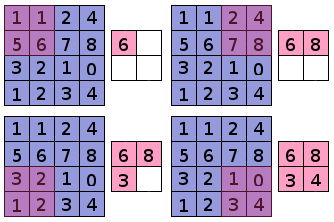
\includegraphics[width=200px]{pooling.png}
   \caption{Ejemplo de max pooling sobre un feature map, con un receptive field de 2 y un stride de 2.}
  \label{fig:pooling}
\end{figure}

Al reducir la dimensionalidad de cada feature map, el pooling hace más manejable las representaciones, reduce el número de parámetros y computaciones en la red y ayuda a llegar a una representación de la imagen invariante con respecto a pequeñas traslaciones.

\subsubsection{Capa de introducción de no-linearidad}

La mayoría de los problemas que queremos modelar con una red convolucional son de carácter no lineal. Dado que la convolución es una operación lineal es necesario introducir una capa de no linearidad.

Para el paso de no linearidad se utiliza la operación ReLU. ReLU es una operación que se aplica píxel por píxel, reemplazando todos los valores negativos de un feature map por cero. Se pueden utilizar otras funciones de no linearidad como $tanh$ o $sigmoida$, pero las funciones rectificadoras (ReLU, Leaky ReLU) son las que mejor funcionan en la mayoría de los casos.


\section{Inception Score} \label{inception_score}

El inception score \cite{inception_score} \cite{pros_cons_gan_evaluation} es uno de los métodos más adoptados para medir la calidad generativa que tiene una GAN. Utiliza una red neuronal pre-entrenada sobre el dataset ImageNet \cite{imagenet_cvpr09} para capturar propiedades deseables de los ejemplos generados: deben contener objetos claramente visibles (por ejemplo, deben ser enfocadas en lugar de difusas) y tener gran diversidad.

El método muestra una correlación razonable con la calidad y la diversidad de las imágenes generadas como así también con la evaluación realizada por humanos. Cuando se calcula sobre los datos de entrenamiento puede servir como cota superior.

A pesar de ser una de las técnicas más utilizadas para medir la calidad de las muestras, tiene algunos problemas:

\begin{itemize}
\item  No es capaz de detectar sobreajuste. Puede ser fácilmente engañado por un modelo que haya memorizado un subconjunto de los datos de entrenamiento.
\item Es muy sensible a la resolución de las imágenes que evalúa.
\item Puede favorecer modelos que generan buenos objetos antes que imágenes realistas.
\end{itemize}



\section{Trabajos relacionados}

A continuación se describirán estudios que fueron la base o una fuente de inspiración para el presente trabajo.\\

Existen técnicas para mejorar los resultados de generadores en entrenamientos sin supervisión sobre datasets de alta variabilidad. En el trabajo de David Warde-Farley et al. \cite{warde-farley+al-2017-denoisegan-iclr} se propone un método de entrenamiento de GAN que ataca algunas deficiencias de la formulación original. Se considera al discriminador como una potencial fuente de información complementaria sobre los datos de entrenamiento. La distribución de las activaciones de alto nivel del discriminador cuando son evaluadas pueden ser utilizadas como una fuente adicional de conocimiento acerca de distribución de datos. La forma de rastrear dicha distribución es a través de un \textit{denoising auto-encoder} \footnote{Un autoencoder es un tipo de red que aprende a comprimir datos introducidos en la capa de entrada y luego a descomprimirlos de forma tal que la salida esté muy cerca de los datos de entrada.} entrenado sobre las capas ocultas del discriminador cuando se evalúan los datos de entrenamiento. La información obtenida se utiliza para proponer nuevos objetivos de alto nivel para el generador.

Han Zhang et al. proponen un modelo llamado Self-Attention Generative Adversarial Network (SAGAN) \cite{2018arXiv180508318Z} el cual introduce un mecanismo de auto-atención (un mecanismo de atención indica a la red dónde ``mirar'' cuando ésta intenta predecir o generar partes de una secuencia) en las GANs. El módulo de auto-atención es complementario a las convoluciones y ayuda a modelar dependencias de multi nivel y de largas distancias a través de las regiones de una imagen. Este mecanismo permite que el generador pueda dibujar imágenes en donde los detalles finos de cada región están coordinados con detalles finos en porciones distantes de la imagen.

Otro trabajo que tiene como objetivo mejorar la estabilidad y la variabilidad de las GAN es el de Tero Karras et al. \cite{DBLP:journals/corr/abs-1710-10196}. Este trabajo propone incrementar la resolución de las imágenes de manera progresiva durante el entrenamiento. Se comienza con una resolución muy baja, y a medida que avanza el entrenamiento se van agregando capas que posibilitan ir incrementando la resolución. Este incremento le permite a la red descubrir primero características de gran escala en la distribución de imágenes para luego hilar más fino en caracterizaciones detalladas encontradas en resoluciones más grandes, en lugar de tener que aprender todas las caracterizaciones de forma simultánea.

Yuri Ostrovsky et al. \cite{visual_parsing} realizaron experimentos con humanos que luego de un tratamiento para recuperar la visión, mostraron muchas dificultades a la hora de interpretar imágenes estáticas en las primeras etapas de entrenamiento visual. Se observaron problemas para tareas básicas de reconocimiento como el agrupamiento de partes y la detección de continuidad y unión de un objeto. Por otro lado, al recibir estímulos de imágenes en movimiento se encontró que no sólo segmentaron figuras de forma correcta, sino que con el tiempo también desarrollaron la habilidad de interpretar adecuadamente imágenes fijas. Estos resultados sugieren que el movimiento juega un papel fundamental en tareas de segmentación y reconocimiento de objetos.

Los conjuntos de píxeles que conforman un objeto en una imagen pueden variar en textura y color, es decir, no siempre está formado por píxeles de una sola familia de colores, ni tampoco tiene una textura uniforme. Al no tener información de cuál es el objeto a enfocar, una red tiene un trabajo más difícil en aprender conceptos de alto nivel como su forma y pose, quedándose sólo con representaciones que conforman el objeto por separado.

En el trabajo realizado por Deepak Pathak et al. \cite{learning_features} se muestra que una red convolucional puede aprender buenas representaciones cuando se la entrena para segmentar a partir de imágenes manualmente segmentadas de alta calidad (obtenidas del dataset COCO \cite{coco}), sin usar etiquetas de clase. Utilizando transfer learning, se mostró que las caracterizaciones aprendidas fueron muy efectivas para la detección de objetos.

Otro resultado obtenido por ellos fue el de emplear imágenes algorítmicamente segmentadas sin ningún tipo de supervisión sobre el dataset YFCC100m (Yahoo Flickr Creative Commons 100 million \cite{yfcc100m}). Utilizando transfer learning para la detección de objetos luego del entrenamiento con este dataset sigue habiendo una buena performance, teniendo mejores resultados que otros métodos sin supervisión.

Los experimentos descriptos nos llevan a suponer que dada una red entrenada con el propósito de aprender a segmentar, teniendo como entrada segmentaciones de alta calidad, puede obtener buenas caracterizaciones. 

\chapter{Experimentos}

En este capítulo se verán en detalle los datasets, las arquitecturas utilizadas para la realización de los experimentos y se hará un análisis de los resultados obtenidos.

\section{Datasets}


De cada dataset sin procesar se obtuvieron como base dos datasets, uno con imágenes con los tres canales estándares y otro con los tres canales estándares y su máscara de segmentación correspondiente como un canal extra.

Las herramientas utilizadas en la preparación de los dataset fueron OpenCV \cite{opencv_library} para la separación/mezcla de canales y redimensionado de las imágenes, NumPy \cite{numpy} para el manejo de arreglos y matrices y h5py \cite{h5py} para guardar las estructuras de datos en archivos.

Todas las imágenes como así también sus máscaras fueron redimensionadas a 64 píxeles de ancho por 64 píxeles de alto utilizando la interpolación por área, la cual nos da una mayor calidad y menor pérdida de información al achicar. Las máscaras fueron llevadas a la escala de los canales RGB (en el intervalo $[0, 255]$). El resultado de este proceso para una imagen es un arreglo multidimensional de enteros de 8 bits sin signo (enteros de 0 a 255), donde las primeras dos dimensiones son el alto y el ancho respectivamente y la tercer dimensión la cantidad de canales. Luego del procesamiento, las imágenes se organizan en un arreglo de NumPy y se guardan en un archivo.

\subsection{Yahoo Flickr Creative Commons}

Yahoo Flickr Creative Commons 100 million (YFCC100m) \cite{yfcc100m} es un dataset con un total de 100 millones de objetos multimedia. Del total, 99.2 millones son fotografías y 0.8 millones son videos. El contenido fue subido por usuarios de la red Flickr, publicados bajo la licencia Creative Commons.

En el dataset existen 68.552.616 fotos y 418.207 videos los cuales tienen etiquetas añadidas por usuarios, correspondientes a distintas categorías y subcategorías (por ejemplo en la categoría \textit{personas} existen las etiquetas \textit{bebé, familia,} etc...). Además, también cuenta con 3.343.487 fotos y 7.281 videos con anotaciones generadas automáticamente por algún sistema.

De todo el dataset sólo se utilizaron los videos sin tener en cuenta sus etiquetas. La segmentación fue realizada por Deepak Pathak et al. \cite{learning_features} y publicada para su uso \footnote{\url{https://people.eecs.berkeley.edu/~pathak/unsupervised_video/}}. Para segmentar los videos utilizaron una modificación del algoritmo NLC \cite{nlc}, llamada uNLC que reemplaza un detector de bordes entrenado con datos etiquetados por segmentación basada en superpíxeles \footnote{Un superpíxel es una aglomeración de píxeles adyacentes con colores o niveles de gris similares.}.
En primer lugar, uNLC computa un mapa de prominencia \footnote{Un mapa de prominencia es una simplificación de una imagen. El objetivo de esta simplificación es resaltar características significativas de interés y facilitar el análisis.} (Figura \ref{fig:silency_map}) basado en movimiento de cada uno de los fotogramas. Existen dos criterios para computar este mapa:

\begin{itemize}
\item Observar los píxeles que se mueven en una escena mayoritariamente estática. 
\item Si la escena contiene mucho movimiento, observar los píxeles que se mueven en direcciones diferentes al promedio. 
\end{itemize}

\noindent Luego, se calcula la media de la prominencia de cada uno de los píxeles dentro de una región delimitada por un superpíxel. Esto se hace por cada superpíxel. En el próximo paso se computa un grafo de vecinos más cercanos sobre los superpíxeles del video usando ubicación y apariencia como características. Finalmente, se utiliza el algoritmo de votación de vecinos más cercanos sobre un grafo de regiones que tienen características similares (color, estructura local) para propagar la prominencia a través de los fotogramas.

\begin{figure}[H]
\centering
 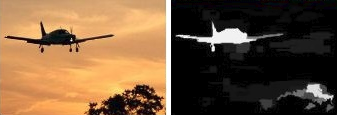
\includegraphics[width=200px]{silency_map.png}
   \caption{Ejemplo de un mapa de prominencia. A la izquierda la imagen original y a la derecha su mapa de prominencia correspondiente (basado en contraste).\protect\footnotemark}
  \label{fig:silency_map}
\end{figure}
\footnotetext{Imagen tomada de \url{http://geometry.cs.ucl.ac.uk/projects/2014/globalContrast/}.}

Los videos fueron separados en distintas tomas antes de segmentarlos con uNLC. Para descartar malas segmentaciones se utilizaron dos heurísticas:

\begin{enumerate}
\item Descartar fotogramas con muchos (mayor al 80\%) o muy pocos (menor al 10\%) píxeles marcados como el objeto a enfocar.
\item Descartar fotogramas con muchos píxeles (mayor al 10\%) con el 5\% del borde marcados como el objeto a enfocar.
\end{enumerate}

El algoritmo se corrió sobre 205.000 videos. Se extrajeron entre 5 y 10 fotogramas por toma obteniendo así un dataset de 1.6 millones de imágenes. De cada fotograma se produjeron dos imágenes: una común de tres canales y otra de un solo canal, con valores de 0 a 100 representando la máscara del fotograma, donde los valores más cercanos a 100 representan una mayor probabilidad de que dicho píxel sea parte del objeto en movimiento. En la Figura \ref{fig:ejemplo_unlc} se puede ver el resultado final sobre un fotograma. En este proceso, la segmentación sólo se limita a separar lo que está en movimiento del resto. Por ejemplo, si en una escena hay dos personas caminando, el algoritmo separará del fondo a las dos personas como un objeto único y no a cada una como dos segmentaciones diferentes. Esto se puede ver en la Figura \ref{fig:unlc_overlap}. 

\begin{figure}[H]
\centering
 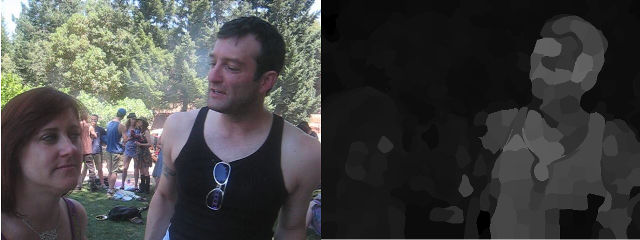
\includegraphics[width=\linewidth]{ejemplo_unlc.jpg}
   \caption{Segmentación de un fotograma utilizando el algoritmo uNLC. A la izquierda, la imagen de tres canales correspondiente al fotograma. A la derecha, la probabilidad de cada píxel de ser parte del objeto enfocado. Las áreas oscuras representan una menor probabilidad mientras que las áreas claras una mayor probabilidad.}
  \label{fig:ejemplo_unlc}
\end{figure}


\begin{figure}[H]
\centering
 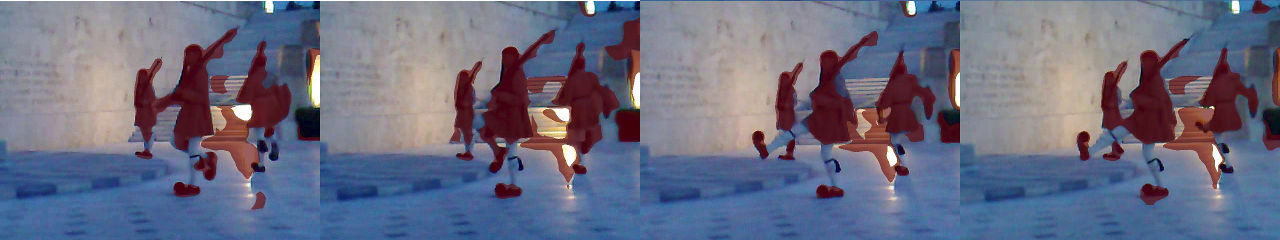
\includegraphics[width=\linewidth]{overlap.jpg}
   \caption{Muestra de la segmentación hecha por uNLC en fotogramas consecutivos. La máscara roja representa el enfoque hecho por el algoritmo sobre los fotogramas.}
  \label{fig:unlc_overlap}
\end{figure}
\newpage
\subsubsection{Preparación}


Partiendo de las imágenes y segmentaciones obtenidas por Deepak Pathak et al. éstas se filtraron utilizando una versión modificada del código de ejemplo de clasificación de imágenes de Tensorflow \footnote{\url{https://github.com/tensorflow/models/blob/master/tutorials/image/imagenet/classify_image.py}} con una red neuronal entrenada sobre ImageNet para mil clases \footnote{\url{http://image-net.org/challenges/LSVRC/2014/browse-synsets}}. En el algoritmo de clasificación sólo se evaluaron las imágenes con los tres canales estándares, dado que la máscara no aporta información importante para esta tarea.
\enlargethispage{0.9in}

Para seleccionar una imagen, la misma debe tener un 75\% de probabilidades como mínimo de pertenecer a una de las mil clases antes mencionadas. El propósito del filtrado es reducir lo más posible el ruido para poder evaluar el modelo en presencia y ausencia de éste.

Como resultado, de 1.618.792 muestras sólo quedaron 207.103. Estas fueron las imágenes utilizadas para obtener los datasets a procesar. De las imágenes sin filtrar también se obtuvieron los datasets correspondientes. En la Figura \ref{fig:comparacion_datasets_normales} se puede ver una fracción del arreglo de imágenes resultante.

\begin{figure}[H]
\centering
 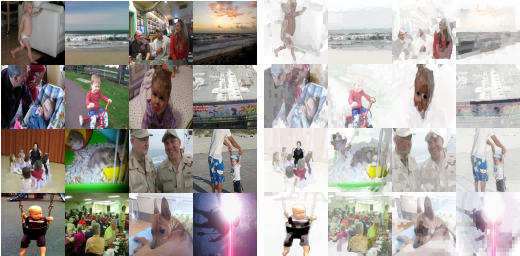
\includegraphics[width=\linewidth]{comparacion_datasets_normales.png}
   \caption{Datasets resultantes. A la izquierda, el dataset conformado por imágenes con los tres canales estándares. A la derecha, el dataset con conformado por imágenes con los tres canales estándares y su máscara de segmentación correspondiente. Para poder visualizar las imágenes con cuatro canales, se tomó el canal correspondiente a la máscara como el canal alfa de una imagen convencional.}
  \label{fig:comparacion_datasets_normales}
\end{figure}


\subsection{Microsoft COCO}

Microsoft Common Objects in Context (MS COCO) \cite{coco} es un dataset con un total de 328.000 imágenes que contienen 91 clases de objetos categorizados, teniendo más de 5.000 instancias de 82 de las categorías. En total, el dataset cuenta con 2.5 millones de etiquetas.

Uno de los objetivos del dataset es que la mayor parte de las imágenes no sean icónicas. Una imagen se considera icónica cuando sólo contiene un objeto grande en el centro de la misma (Figura \ref{fig:iconic_vs_noiconic}). La elección de este tipo de imágenes se debe a que, si bien las imágenes icónicas proveen una muestra de alta calidad de los objetos, carecen de información contextual importante y de distintos puntos de vista.

\begin{figure}[H]
\centering
 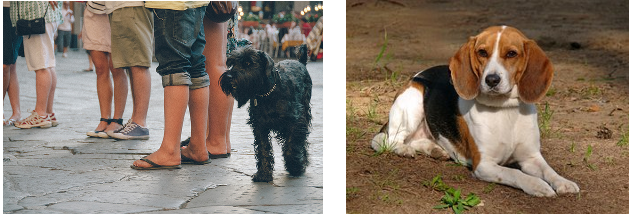
\includegraphics[width=\linewidth]{iconic_vs_noiconic.png}
   \caption{A la izquierda, una imagen no icónica de un perro. A la derecha, una imagen icónica de un perro.}
  \label{fig:iconic_vs_noiconic}
\end{figure}

Las imágenes fueron clasificadas, anotadas y segmentadas por humanos. La primer tarea es determinar qué categorías de objetos están presentes en cada imagen. Para hacer esto, primero se agruparon las categorías de objetos en 11 supercategorías (por ejemplo, los objetos \textit{perro, gato, pájaro}, etc... se agrupan en la supercategoría \textit{animal}). Para una imagen en particular, un trabajador humano debe indicar qué supercategorías están presentes, para luego marcar las categorías concretas. Dado que una imagen puede tener más de una instancia de una determinada categoría, la segunda tarea se trata de marcar todas las instancias de las categorías encontradas en la primer etapa. Para realizar esto, un trabajador debe marcar con cruces que varían en color dependiendo su categoría cada objeto encontrado. La última tarea, es segmentar a mano las instancias de los objetos, siguiendo como guía las cruces puestas en la etapa previa. El proceso se puede ver en la Figura \ref{fig:proceso_segmentacion}.

Como resultado se obtiene un dataset variado, compuesto mayoritariamente por imágenes no icónicas las cuales ayudan a la generalización y con segmentaciones de altísima calidad.

\begin{figure}[H]
\centering
 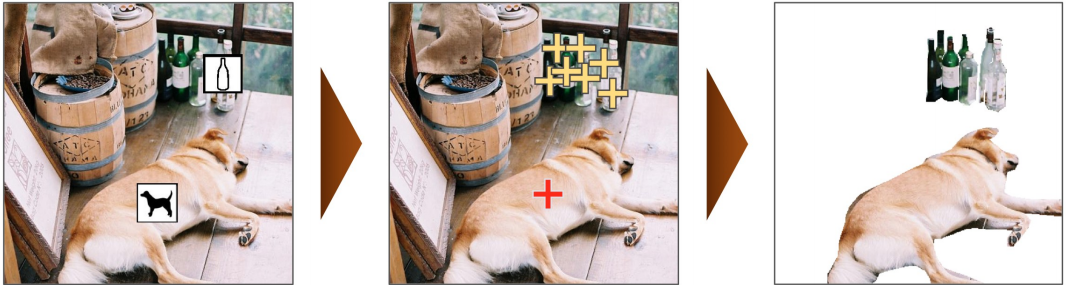
\includegraphics[width=\linewidth]{proceso_segmentacion.png}
   \caption[Proceso de clasificación, anotación y segmentación de una imagen para el dataset COCO.]{Proceso de clasificación, anotación y segmentación de una imagen para el dataset COCO \protect\footnotemark}
  \label{fig:proceso_segmentacion}
\end{figure}

\footnotetext{Imagen tomada del paper original \cite{coco}.}

\subsubsection{Preparación}

No se excluyó ninguna categoría de las 91 disponibles. Si en una imagen hay más de una categoría de objetos presente, se toma cada instancia por separado, generando tantas imágenes segmentadas como objetos categorizados presentes en la imagen original. 

Las imágenes y sus metadatos se obtuvieron utilizando la API de COCO \footnote{\url{https://github.com/cocodataset/cocoapi}} de forma completamente aleatoria. Estas se procesaron en su tamaño original al momento de generar las segmentaciones. Para producir las imágenes segmentadas, se tradujo el polígono que marca el contorno de una instancia de un objeto en un canal alfa, donde los píxeles contenidos dentro del área del polígono toman el valor 255 mientras que los píxeles situados fuera del área toman el valor 0. Debido a que luego se redimensionan a 64x64 píxeles, no se toman en cuenta aquellas cuya segmentación no está formada por al menos un 15\% de área total de píxeles. Este tipo de imágenes se ignoran porque no aportan de manera significativa al dataset debido a que al redimensionarlas a una resolución tan baja, la pérdida de información es muy grande.

Como resultado, de 58.386 imágenes se obtuvieron 77.882 segmentaciones. En la Figura \ref{fig:comparacion_datasets_coco} se puede ver una fracción del arreglo de imágenes resultante.

\begin{figure}[H]
\centering
 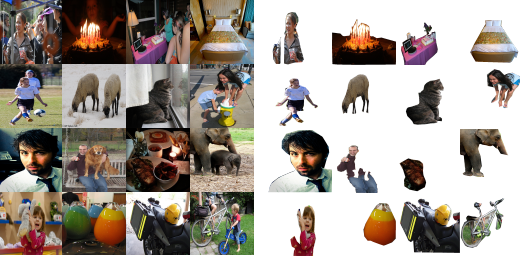
\includegraphics[width=\linewidth]{comparacion_datasets_coco.png}
   \caption{Datasets resultantes. A la izquierda, el dataset conformado por imágenes con los tres canales estándares. A la derecha, el dataset con conformado por imágenes con los tres canales estándares y su máscara de segmentación correspondiente.}
  \label{fig:comparacion_datasets_coco}
\end{figure}

\section{Arquitectura}

La profundidad de la red es un aspecto muy importante con respecto a su arquitectura. A medida que las redes se van haciendo cada vez más profundas, se vuelven más difíciles de entrenar. Tanto el generador como el discriminador que se utilizan en todas las pruebas están construidos como una Residual Network (ResNet) \cite{resnet_paper} \cite{resnet_1}, las cuales nos permiten construir redes más profundas con un número similar de parámetros. 
\newpage
Como demostró Kaiming He et al. en su tabajo ``Convolutional Neural Networks at Constrained Time Cost'' \cite{DBLP:journals/corr/He014} cuando la profundidad de la red crece, llega un punto en que en lugar de mejorar su precisión ésta se satura, es decir, el entrenamiento se frena o se mueve muy lento. Este problema no se debe al sobreajuste y agregar más capas deriva en un error de entrenamiento más alto.

%Saturated nodes lead to a situation where a small change in the input-to-hidden weights during training will likely not change the sum-of-products very much, and then after activation, the node value will still be -1.0 or +1.0 — in other words, training stalls out or moves very slowly. Additionally, saturated models are often overfitted — meaning the model predicts well on training data but poorly on new, unseen data.

Las ResNet utilizan lo que se conoce como \textit{Residual Block} (Figura  \ref{fig:residual_block}). Un \textit{Residual Block} aglomera un conjunto de capas y agrega una conexión llamada \textit{shortcut} entre la entrada del bloque y un nodo de suma, el cual está ubicado justo antes de la última función de activación previo a salir del bloque.

\begin{figure}[h]
\centering
 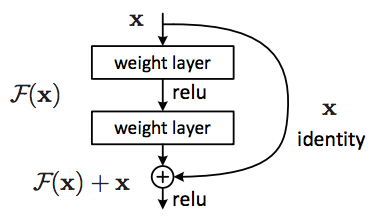
\includegraphics[width=200px]{resiudal_block.png}
   \caption[Representación de un residual block.]{Representación de un residual block. \protect\footnotemark}
  \label{fig:residual_block}
\end{figure}

\footnotetext{Imagen tomada del paper original \cite{resnet_paper}.}

\noindent Esta conexión en principio es la función identidad. Una capa, en una red neuronal ``plana'' toma su entrada y calcula su salida como $y = \mathcal{F}(x)$. En contraste, un \textit{residual block} en una ResNet calcula $y = \mathcal{F}(x) + x$. Los \textit{shortcuts} en conjunto con el nodo suma, le da la capacidad a la red de aprender representaciones incrementales. Intuitivamente, se puede pensar que es mejor comprender un concepto teniendo como referencia la base con la que fue elaborado. Una red neuronal profunda puede ser fácilmente convertida en una ResNet agregando shortcuts y nodos suma para crear residual blocks.

A continuación veremos las arquitecturas concretas del generador y del discriminador  utilizados para la experimentación. La función de activación o no-linearidad utilizada siempre es ReLU, a menos que se indique lo contrario. El tamaño de los filtros utilizados en las convolucines es siempre 3 y la cantidad de mapas es siempre 128. El learning rate inicial es de 0.0002.

\subsection{Generador}

El generador está formado por una capa de entrada, cuatro Residual Blocks idénticos, una capa de Batch Normalization y una capa de salida conformada por una convolución y la función de activación \textit{tanh}. Los residual blocks están constituidos de la siguiente manera:

\begin{enumerate}
\item Batch Normalization con aplicación de no-linearidad
\item Convolución
\item Batch Normalization con aplicación de no-linearidad
\item Convolución
\item Nodo suma con un shortcut dado por una convolución en el input en lugar de la función identidad.
\end{enumerate}


\subsection{Discriminador}
\enlargethispage{0.5in}
El discriminador está formado por una capa de entrada, cuatro Residual Blocks con orden R1, R2, R3, R3, aplicación de no-linearidad a la salida del último residual block y una capa de salida. La descripción de los residual blocks se puede ver en el Cuadro \ref{tab:tabla_resblocks}.
\begin{table}[H]
	\resizebox{\textwidth}{!}{
	\begin{tabular}{| l | l | l |}
	  \hline			
	  Residual Block R1 & Residual Block R2 & Residual Block R3 \\
	  \hline  
	  1. Convolución + No-Linearidad & 1. Batch Norm + No-Linearidad & 1. Batch Norm + No-Linearidad  \\
	  2. Convolución & 2. Convolución & 2. Convolución\\
	  3. Nodo suma con Shortcut & 3. Batch Norm + No-Linearidad & 3. Batch Norm + No-	Linearidad \\
	  ~~1- Convolución & 4. Convolución & 4. Convolución~ \\
	  ~~2- Average pooling  & 5. Average pooling & 5. Nodo suma con Shortcut\\
	  ~ & 6. Nodo suma con Shortcut & ~~1- Convolución \\
	  ~ & ~~1- Convolución & ~ \\
	  ~ & ~~2- Average pooling  & ~\\
	  \hline  
	\end{tabular}
	}
\caption{Descripción de los residual blocks utilizados en el discriminador.}\label{tab:tabla_resblocks}
\end{table}

\noindent 

Se utilizó la librería Tensorflow \cite{tensorflow}, capaz de generar código CUDA, para el armado y evaluación de las arquitecturas antes mencionadas. Se tomó como base el código \footnote{\url{https://github.com/igul222/improved_wgan_training}} de Ishaan Gulrajani et al. usado en las pruebas de su trabajo ``Improved Training of Wasserstein GANs'' \cite{improved_wegan_training} 

Se escogió esta arquitectura por ser la que alcanza el estado del arte con CIFAR10.

\section{Entrenamiento}

El entrenamiento se dividió en tres grandes pruebas. La primera, consiste en evaluar el dataset extraído de COCO. Considerando que es un dataset casi sin ruido (porque en cada imagen siempre hay un único objeto que se enfoca, perteneciente a alguna de las clases y con un tamaño apreciable respecto al tamaño total) y las máscaras de segmentación son casi perfectas, los resultados obtenidos darán una buena base para evaluar las pruebas con datasets de menor calidad. La segunda, consiste en evaluar el dataset extraido de YFCC100m filtrado. En este caso se mide qué tanto influyen las segmentaciones en la mejora de la calidad de generación de imágenes, siendo éstas algo inexactas y no binarias. Esto último hace referencia a que no hay un corte perfecto entre el fondo y lo que se quiere enfocar, sino que cada píxel de la máscara representa una probabilidad de que el píxel que lo corresponde en la imagen pertenezca al objeto que se quiere segmentar. Por último, se pretende evaluar el dataset extraído de YFCC100m sin filtrar. Dado que este dataset contiene muchas imágenes que son difíciles de distinguir incluso para un humano, el objetivo es ver en qué medida el ruido afecta la calidad de generación.

En todas las pruebas antes mencionadas, se utilizan tanto el dataset de tres canales como su correspondiente de cuatro canales, para poder ver el impacto de las segmentaciones sobre el mismo conjunto de datos.

Por cada paso de entrenamiento del generador, el discriminador es entrenado cinco veces. El batch size del discriminador es de 64 mientras que el del generador es de 128, los cuales son tamaños suficientemente grandes para poder aprovechar al máximo memoria disponible al momento de experimentación.

Se midió el \textit{inception score} en cada uno de los datasets para tener una cota superior de referencia sobre el puntaje alcanzado en los resultados de la experimentación.

Todas las pruebas fueron corridas sobre el sistema Ubuntu 16.04, con una placa de video NVIDIA 1070GTX, la cual tiene 1920 CUDA cores a una frecuencia de 1506Mhz, y 8Gb de ram GDDR5 sobre el framework CUDA 8.0.

\subsection{Resultados}
\enlargethispage{0.5in}
En esta sección se expondrán los resultados obtenidos. En principio se realizará un análisis entre los resultados de un mismo dataset con y sin máscara de segmentación y luego un análisis transversal de todos los resultados juntos.


\subsubsection{Dataset COCO} \label{resultados_coco}
\enlargethispage{0.4in}
Lo primero que se puede destacar es que en la mayoría de las muestras derivadas del dataset de cuatro canales, la red segmentó de forma perfecta el objeto enfocado, el cual suele ser muy distinto que el fondo en donde está insertado. Esto se puede observar en la Figura \ref{fig:resultado_segmentacion_coco}. Existen casos también en que el fondo no es tan distinguible del objeto, pero en la segmentación se puede ver una forma bien definida, como en la Figura \ref{fig:resultado_segmentacion_coco2}, segunda fila, segunda columna, donde el objeto parece ser un animal y el fondo tierra con árboles, pero el color del animal y del fondo son similares.

\begin{figure}[H]
\centering
 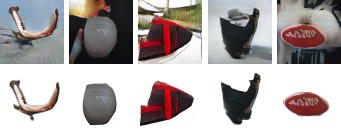
\includegraphics[width=250px]{resultado_segmentacion_coco.jpg}
   \caption{Muestras del resultado del entrenamiento con el dataset COCO de cuatro canales. En la fila superior, las imágenes completas resultantes. En la fila inferior, los objetos enfocados por la red.}
  \label{fig:resultado_segmentacion_coco}
\end{figure}

Es también visible que se logró separar satisfactoriamente algunas clases de entrenamiento más allá de que las redes hayan sido entrenadas sin etiquetas. Esto se puede distinguir gracias a que la proporción y la forma de los objetos está mucho mejor conservada cuando la segmentación está presente que cuando no. En la primera fila de la Figura \ref{fig:resultado_segmentacion_coco2} se pueden observar siluetas humanas bastante bien proporcionadas, con varios cambios de textura y color (cara, ropa) perteneciente al mismo objeto enfocado. 

\begin{figure}[h]
\centering
 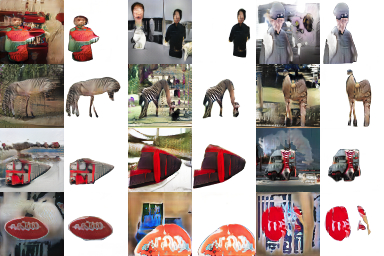
\includegraphics[width=300px]{resultado_segmentacion_coco2.jpg}
   \caption{Muestras del resultado del entrenamiento con el dataset COCO de cuatro canales donde son distinguibles clases de objetos pertenecientes a dicho dataset. En la primer fila, la clase \textit{persona}. En la segunda fila, distintas muestras de la superclase \textit{animal}. En la tercer fila, muestras de la superclase \textit{transporte} (en particular las clases \textit{tren} y \textit{camión}). En la cuarta fila, la clase \textit{cartel de pare}.}
  \label{fig:resultado_segmentacion_coco2}
\end{figure}

\enlargethispage{0.3in}
 En el caso de tres canales, la separación en clases también es observable pero en menor medida, debido a que las muestras en general están menos definidas y en varios casos los objetos parecen fundirse con el fondo por no tener una silueta bien marcada. En la Figura \ref{fig:comparacion_coco_3chan} se puede distinguir lo que parecen ser algunas clases. Por ejemplo, en la primer imagen se puede ver la textura de una cebra, pero con un contorno sin definir y entremezclada con el fondo en la parte izquierda.

\begin{figure}[H]
\centering
 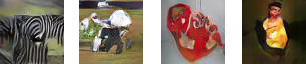
\includegraphics[width=200px]{comparacion_coco_3chan.jpg}
   \caption{Muestras del resultado del entrenamiento con el dataset COCO de tres canales donde parecen distinguirse algunas clases. En las primeras dos imágenes, la superclase \textit{animal} (en particular \textit{cebra} en la primera). En la tercer imagen, la clase \textit{cartel de pare}. En la última imagen, la clase \textit{persona}.}
  \label{fig:comparacion_coco_3chan}
\end{figure}

Es notable que el canal extra que provee la información de enfoque sobre el objeto de interés en una imagen tuvo una importante influencia en los resultados obtenidos. No sólo ayuda a la red a reconocer mejor las clases con las que entrena, sino que además también favorece la interpretación de la forma y pose de dichas clases.

En el Apéndice \ref{apendice:coco} se pueden ver todos los resultados del dataset COCO, de donde fueron extraídas las muestras vistas en esta sección.
 
\subsubsection{YFCC100m filtrado}

Se puede observar que hay más variabilidad con respecto a la segmentación. Hay imágenes donde lo que está segmentado es claramente diferenciable del fondo mientras que en otras no parece distinguirse bien qué es fondo de lo que es un objeto o tienen una segmentación sin sentido. En estas últimas, los valores de la máscara que indican la separación entre lo enfocado y lo no enfocado son mucho más homogéneos en comparación con los de máscaras de imágenes con una buena segmentación, donde el rango entre valores altos y bajos es más grande. En la Figura \ref{fig:resultados_filtrado_segmentacion} se puede observar este fenómeno.

\begin{figure}[H]
\centering
 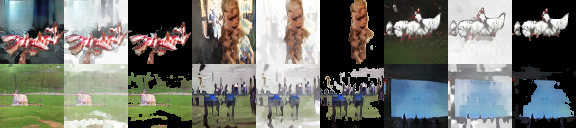
\includegraphics[width=\linewidth]{resultados_filtrado_segmentacion.png}
   \caption{Muestras del resultado del entrenamiento con el dataset YFCC100m filtrado de cuatro canales. En la primer fila, segmentaciones bien enfocadas y diferenciables del fondo. En la segunda fila, segmentaciones difusas y no muy diferenciables del fondo. Por cada imagen tenemos la versión sin el canal alfa, con el canal alfa y con una máscara negra sobre los puntos menos probables (menores al 50\%) de pertenecer al objeto enfocado respectivamente.}
  \label{fig:resultados_filtrado_segmentacion}
\end{figure}

\noindent Otra característica a destacar es que en algunas imágenes los objetos enfocados no parecen tener continuidad sino ser un conjunto de enfoques inconexos. Así mismo, estos enfoques inconexos se suelen agrupar juntos y tienen la misma textura. Esto se puede ver en la Figura \ref{fig:enfoques_inconexos}

\begin{figure}[h]
\centering
 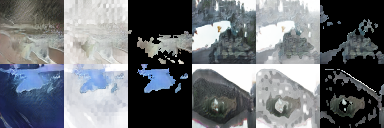
\includegraphics[width=250px]{enfoques_inconexos.png}
   \caption{Muestras del resultado del entrenamiento con el dataset YFCC100m filtrado de cuatro canales. Bloques con enfoques disconexos que mantienen su textura. Por cada imagen tenemos la versión sin el canal alfa, con el canal alfa y con una máscara negra sobre los puntos menos probables (menores al 50\%) de pertenecer al objeto enfocado respectivamente.}
  \label{fig:enfoques_inconexos}
\end{figure}

Estas características se pueden deber a la configuración propia del dataset, donde no hay una diferenciación abrupta entre lo que es un objeto enfocado y el fondo, sumado a que cuando se enfoca algo, no necesariamente corresponde a una clase de objeto en particular, sino que puede corresponder a varios de distintas clases. Esto está íntimamente ligado a cómo se generó el dataset. Por ejemplo, en una escena donde hay una persona caminando junto a su perro, el algoritmo de detección de movimiento marcará como objeto a enfocar a la persona junto con el perro.

Por último, no parece haber formas reconocibles que distingan claramente alguna clase.\\

En el caso del dataset con tres canales tampoco parece haber clases bien definidas o reconocibles. Es notable, sin embargo, que existen varias muestras que ilustran paisajes de una calidad aceptable. En contraste, el dataset de cuatro canales también generó muestras que ilustran paisajes, pero estas presentan menor calidad, menor variabilidad y menor cantidad. Esto se puede ver en la Figura \ref{fig:paisajes_filtered}.

\begin{figure}[h]
\centering
 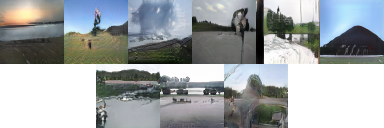
\includegraphics[width=250px]{paisajes_filtered.png}
   \caption{Muestras del resultado del entrenamiento con el dataset YFCC100m filtrado. En la primer fila, paisajes generados con el dataset de tres canales. En la segunda fila, paisajes generados con el dataset de cuatro canales.}
  \label{fig:paisajes_filtered}
\end{figure}
\noindent Es posible que esto se deba a las segmentaciones. Se puede pensar que el hecho de que no estén presentes hace que la red tenga un trabajo más difícil en aprender caracterizaciones más fuertes y definidas sobre los objetos inmersos en esos paisajes.

En el Apéndice \ref{apendice:filtrado} se pueden ver todos los resultados del dataset YFCC100m filtrado, de donde fueron extraídas las muestras vistas en esta sección.

\newpage

\subsubsection{YFCC100m sin filtrar}

Los resultados son muy similares a los obtenidos con YFCC100m filtrado. No parece haber formas reconocibles que distingan claramente alguna clase de objeto. En el dataset de cuatro canales persisten las segmentaciones perfectamente marcadas, las difusas, y los enfoques inconexos. Esto se puede ver en la Figura \ref{fig:resultados_4chan_enter}.

\begin{figure}[h]
\centering
 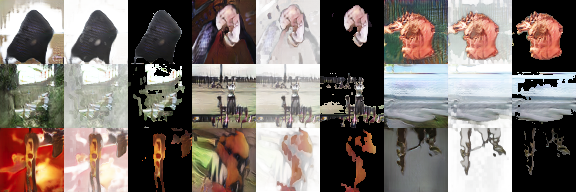
\includegraphics[width=\linewidth]{resultados_4chan_entero.png}
   \caption{Muestras del resultado del entrenamiento con el dataset YFCC100m sin filtrar de cuatro canales.  En la primer fila, segmentaciones bien enfocadas y diferenciables del fondo. En la segunda fila, segmentaciones difusas y no muy diferenciables del fondo. En la tercer fila,  bloques con enfoques disconexos que mantienen su textura. Por cada imagen tenemos la versión sin el canal alfa, con el canal alfa y con una máscara negra sobre los puntos menos probables (menores al 50\%) de pertenecer al objeto enfocado respectivamente.}
  \label{fig:resultados_4chan_enter}
\end{figure}

No hay mucho para destacar del dataset de tres canales. No existen formas distinguibles bien definidas con excepción de algunas muestras que parecen ser de la clase \textit{persona}. Esto se puede ver en la Figura \ref{fig:personas_entero_3ch}. La calidad es baja y las figuras son desproporcionadas, exluyendo las últimas dos. Con cuatro canales no hay manifestaciones de estas formas. Esto se puede deber a que las clases son afectadas de forma negativa por el tipo de segmentación utilizada, o bien en realidad estas muestras no se corresponden con ninguna clase.

\begin{figure}[H]
\centering
 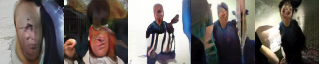
\includegraphics[width=230px]{personas_entero_3ch.png}
   \caption{Muestras del resultado del entrenamiento con el dataset YFCC100m sin filtrar de tres canales de lo que parece ser la clase persona.}
  \label{fig:personas_entero_3ch}
\end{figure}


\noindent En ambos resultados aparecen muestras que aparentan ser paisajes o sitios al aire libre, pero con una calidad bastante baja. Esto se puede ver en la Figura \ref{fig:paisajes_entero}.

\begin{figure}[H]
\centering
 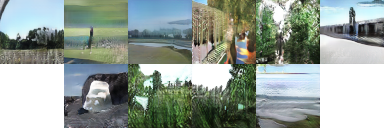
\includegraphics[width=250px]{paisajes_entero.png}
   \caption{Muestras del resultado del entrenamiento con el dataset YFCC100m sin filtrar. En la primer fila, paisajes generados con el dataset de tres canales. En la segunda fila, paisajes generados con el dataset de cuatro canales.}
  \label{fig:paisajes_entero}
\end{figure}

En el Apéndice \ref{apendice:sin_filtrar} se pueden ver todos los resultados del dataset YFCC100m sin filtrar, de donde fueron extraídas las muestras vistas en esta sección.

\subsubsection{Comparativa general}

Es claro que las imágenes obtenidas a partir del entrenamiento con el dataset COCO tienen mejor calidad que las obtenidas con YFCC100m. Es importante destacar que no sólo la presencia de las segmentaciones influye en la generación de imágenes, sino que la calidad de las mismas juega un rol fundamental. Observando tanto los resultados de COCO como los de YFCC100m, se puede ver que la red aprende a separar el fondo de un objeto de interés, obteniendo resultados mucho mejores cuando la calidad de las segmentaciones es alta.

Otro punto a tener en cuenta es la cantidad de objetos enfocados por muestra. En COCO siempre se enfoca un único objeto mientras que en YFCC100m existen tanto imágenes con un único objeto enfocado como con múltiples objetos encuadrados en una misma segmentación. Esto es producto de cómo están constituidos los datasets.

No existe una diferencia notable entre YFCC100m filtrado y no filtrado. Aún así, el filtrado parece haber impactado de forma positiva sobre los resultados, dado que tanto los paisajes como las texturas en general aparentan estar mejor logradas.

Se utilizó el inception score para medir la calidad de los generadores entrenados por ser una métrica que suele correlacionarse bien con la evaluación hecha por humanos. En el Cuadro \ref{tab:inception_scores} se exponen los puntajes obtenidos con cada uno de los datasets. Cabe destacar que para el caso de los datasets con cuatro canales, el inception score se midió sobre los tres canales convencionales.

\begin{table}[H]
\centering

\begin{tabular}{ l | c | c | c }

  ~ & \textbf{Dataset de entrenamiento} & \textbf{3 canales} & \textbf{4 canales}\\
  \hline  
  COCO & $13.51 \pm 0.11$  & $7.37 \pm 0.07$ & $7.50 \pm 0.07$ \\
  YFCC100m filtrado & $22.76 \pm 0.14$ & $8.01 \pm 0.08$ & $7.80 \pm 0.10$ \\
  YFCC100m sin filtrar & $11.75 \pm 0.04$ & $7.53 \pm 0.07$ & $7.06 \pm 0.10 $ \\
  
  
  %%COCO & $13.519704 \pm 0.108648$ & $7.374588 \pm 0.072248876$ & $7.5117836 \pm 0.067126445$ \\
  %%YFCC100m filtrado $22.759604 \pm 0.14101943$ & $8.0197315 \pm 0.082126945$ & $7.7865782 \pm 0.1001841$&  \\
  %%YFCC100m sin filtrar & $11.747463 \pm 0.036891647$ & $7.5318718 \pm 0.074633837 $& $7.0612869 \pm 0.099303342$ \\

\end{tabular}

\caption{Inception score obtenido de los entrenamientos y de los datasets utilizados para los mismos.}\label{tab:inception_scores}
\end{table}

En el cuadro se observa que las muestras de cuatro canales tienen un puntaje mayor sólo con el dataset COCO, lo cual sugiere que el tipo de segmentación utilizada en YFCC100m (no segmentar sólo un objeto de interés, segmentación no-binaria e inexacta) perjudica el proceso de aprendizaje de conceptos. Aún así, la diferencia de puntaje entre cuatro y tres canales de COCO es mínima, aunque las muestras de cuatro canales parecen ser de una calidad notablemente superior. 

Con respecto al ruido en YFCC100m, el hecho de haber realizado un filtrado tuvo como consecuencia que el dataset se acote a las clases reconocibles por la red utilizada para procesar el mismo. Esto nos da una mayor concentración de imágenes pertenecientes a clases específicas y la eliminación de muestras irreconocibles incluso para un evaluador humano. Dado que el inception score es mayor habiendo filtrado el dataset, se puede pensar que el filtrado impactó de forma positiva en el aprendizaje. 

El alto puntaje en YFCC100m filtrado de entrenamiento se puede deber a que éste se procesó con la misma red neuronal utilizada para la medición del inception score. Es probable que esto también haya tenido influencia en el puntaje de los resultados obtenidos a partir del entrenamiento con dicho dataset.


\chapter{Conclusiones y trabajos futuros}

%%es notable que las segmentaciones mejoran las cosas

%% pero cuando la calidad de la segmentación es mas alta y se enfoca un solo objeto la red aprende mejor las caracteristicas

%% Como los resultados son similares en yfcc filtrado y no, entonces es mas de como se segmenta que del ruido al parecer

%% la forma en como esta segmentada parece empeorar las cosas (yfcc)

\section{Conclusiones}

A lo largo de este trabajo se utilizaron redes neuronales profundas generativas de forma no supervisada, para estudiar el impacto que tiene la información dada por la segmentación entre un objeto y el fondo en datasets con alta variabilidad sobre el aprendizajes de características de alto nivel, con el objetivo de generar imágenes artificiales de mayor calidad.

Las pruebas se realizaron con segmentaciones casi perfectas, enfocadas en un solo objeto de interés (derivadas del dataset COCO) y con segmentaciones imperfectas, con uno o varios objetos de interés enfocados en una misma imagen (derivadas del dataset YFCC100m).

Los resultados parecen sugerir que las segmentaciones hacen un aporte significativo al aprendizaje de conceptos de alto nivel dado que las imágenes obtenidas con el dataset COCO de cuatro canales aparentan preservar la forma y pose de las clases aprendidas de manera aceptable. Además, la calidad de las segmentaciones manifiestan ser de gran importancia dado que los resultados producidos con YFCC100m de cuatro canales (tanto filtrado como no filtrado) se presentan menos definidos en comparación con los resultados de COCO y no asignables a una categoría específica.

Otro punto a tener en cuenta es que, si bien luego del filtrado parece haber una mejoría, ésta no es significativa ya que los resultados son muy similares a los no filtrados, por lo que se puede pensar que acotar las clases con las que se entrena tiene menos peso que tener una buena calidad en las segmentaciones.

Es claro que los resultados con COCO de cuatro canales sugieren tener una calidad superior a todos los demás (incluyendo YFC100m filtrado de cuatro canales y COCO de tres canales), lo cual no se refleja en los inception scores obtenidos. Esto se puede deber a que el análisis manual es intrínsecamente subjetivo, es decir, el evaluador humano está sesgado por lo que espera encontrar conociendo las condiciones en las que se realizaron las pruebas, o bien, el inception score es una medida de calidad de generación objetiva que dista de ser perfecta para estos resultados debido a los problemas comentados en la sección \ref{inception_score}.

\section{Trabajos futuros}

Existen tareas que se pueden realizar para continuar la investigación por esta línea de trabajo.

\begin{itemize}
\item Repetir las experiencias realizadas en esta tesina con los datasets etiquetados: Teniendo en cuenta que el entrenamiento supervisado da mejores resultados que el no supervisado, es probable que agregando etiquetas a cada objeto enfocado, la red disponga de mejores herramientas para aprender los conceptos de alto nivel que los conforman.


\item Utilizar una mayor cantidad de mapas en las redes para mejorar su capacidad: Al darle a la red más mapas hacemos que su capacidad de aprendizaje sea mayor. Se pretende que esto impacte de forma positiva a la hora de aprender nuevas características o mejorar las que se pueden aprender con un menor número de mapas. El efecto esperado para este experimento es un aumento en el nivel de detalle en datasets de características similares a COCO y una mejora en el aprendizaje de características para datasets similares a YFC100m filtrado.

\item Utilizar únicamente los objetos enfocados quitando toda la información referente al fondo en cada imagen: Despojar la información innecesaria puede ayudar a la red a centrarse más en los detalles de los objetos enfocados, derivando en un mejor aprendizaje de sus características de alto nivel. La contra cara de este experimento es que, al entrenar la red con imágenes que carecen de información contextual, los resultados serán también carentes de contexto. %% el fundamento de esto es que los filtros que se encargan de reconocer cosas para el fondo ahora se pueden usar para los objetos enfocados.
\end{itemize}



\appendix
\chapter{Resultados del dataset COCO}\label{apendice:coco}
\begin{figure}[H]
\centering
 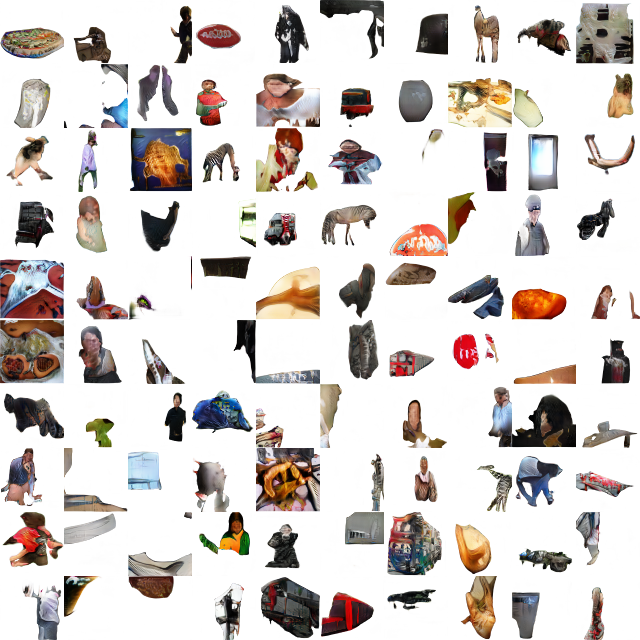
\includegraphics[width=\linewidth]{resultados/coco_4chan_normal.png}
   \caption{Muestras resultante del dataset COCO de cuatro canales.}
  \label{fig:resultado_coco1}
\end{figure}

\begin{figure}[h]
\centering
 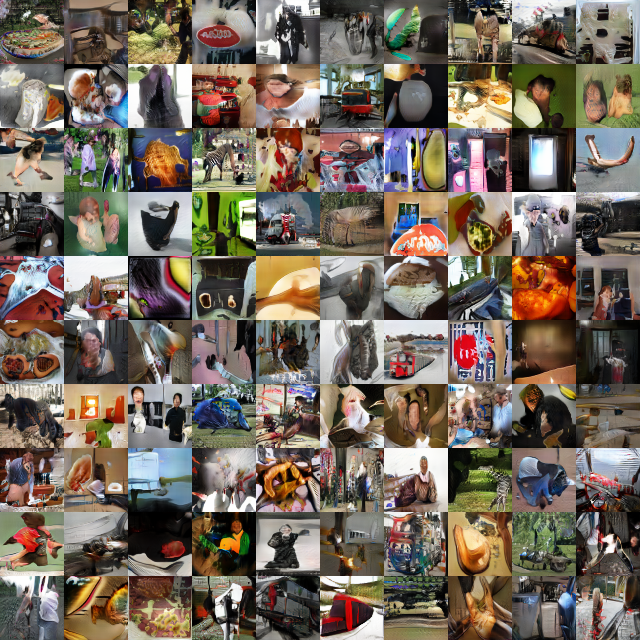
\includegraphics[width=\linewidth]{resultados/coco_4chan_noalpha.png}
   \caption{Muestras resultante del dataset COCO de cuatro canales sin el canal alpha.}
  \label{fig:resultado_coco2}
\end{figure}

\begin{figure}[h]
\centering
 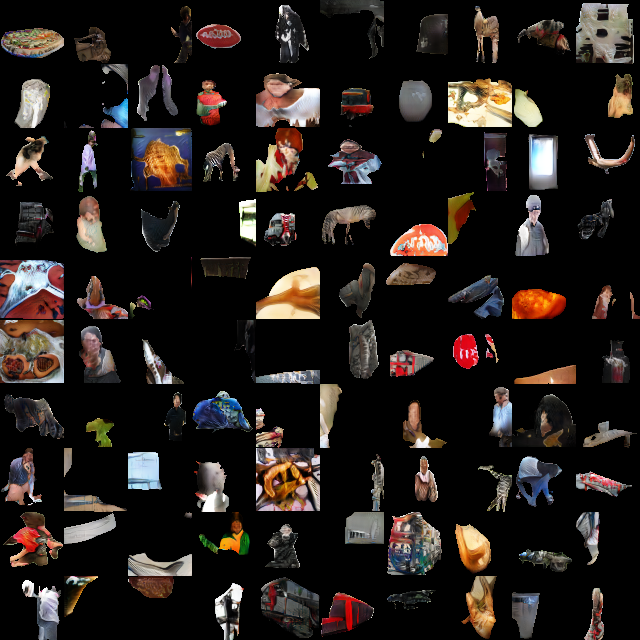
\includegraphics[width=\linewidth]{resultados/coco_4chan_mask.png}
   \caption{Muestras resultante del dataset COCO de cuatro canales aplicando una máscara negra sobre el fondo del objeto enfocado.}
  \label{fig:resultado_coco3}
\end{figure}

\begin{figure}[h]
\centering
 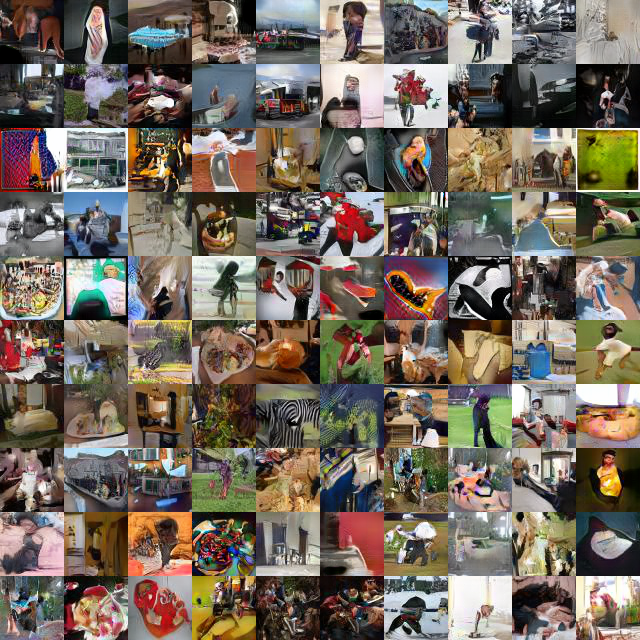
\includegraphics[width=\linewidth]{resultados/coco_3chan.png}
   \caption{Muestras resultante del dataset COCO de tres canales.}
  \label{fig:resultado_coco4}
\end{figure}


\chapter{Resultados del dataset YFCC100m (filtrado)}\label{apendice:filtrado}
\begin{figure}[H]
\centering
 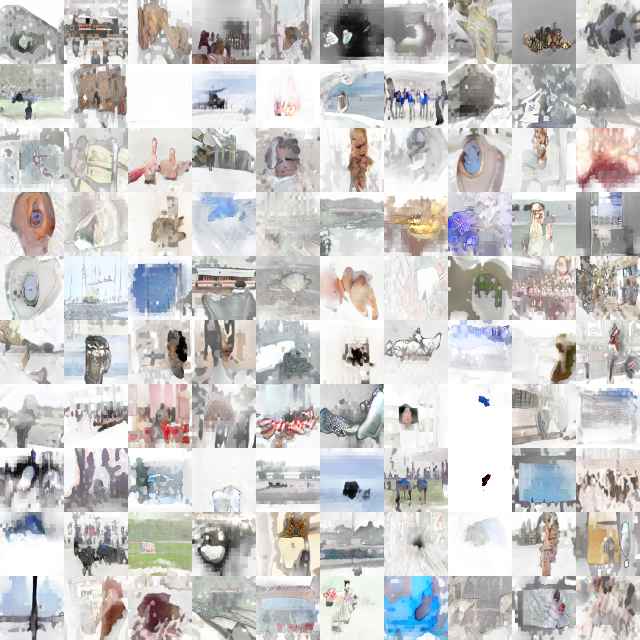
\includegraphics[width=\linewidth]{resultados/filtered_4chan_normal.png}
   \caption{Muestras resultante del dataset YFCC100m filtrado de cuatro canales.}
  \label{fig:resultado_filtrado1}
\end{figure}

\begin{figure}[h]
\centering
 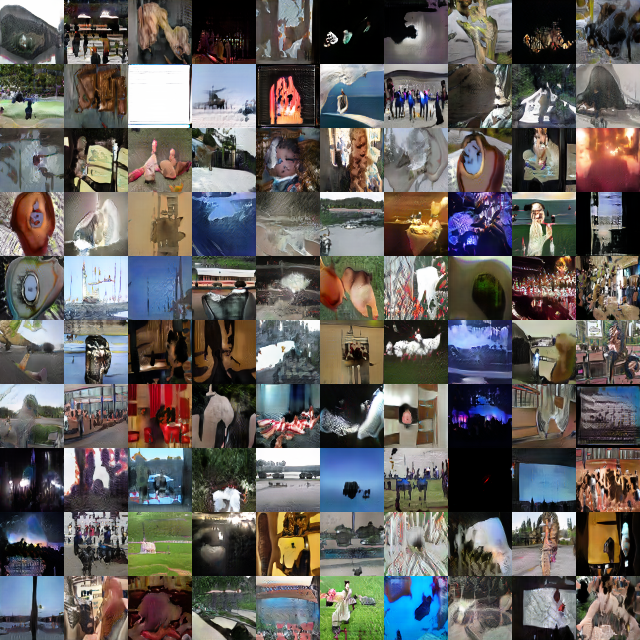
\includegraphics[width=\linewidth]{resultados/filtered_4chan_noalpha.png}
   \caption{Muestras resultante del dataset YFCC100m filtrado de cuatro canales sin el canal alpha.}
  \label{fig:resultado_filtrado2}
\end{figure}

\begin{figure}[h]
\centering
 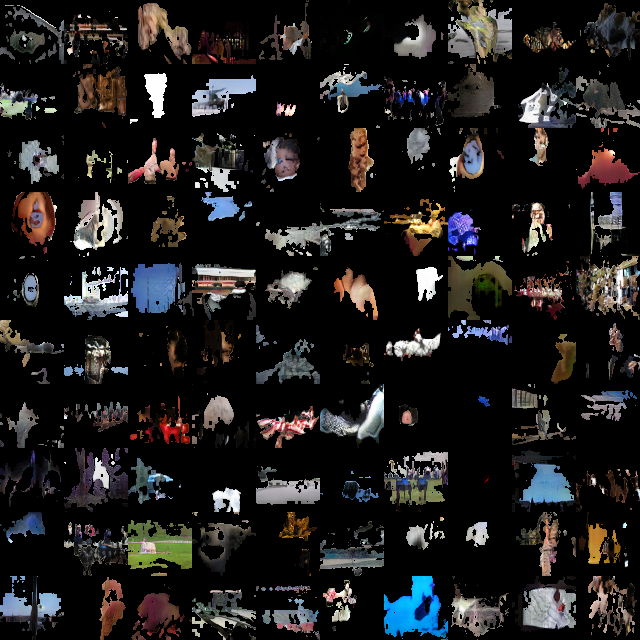
\includegraphics[width=\linewidth]{resultados/filtered_4chan_mask.png}
   \caption{Muestras resultante del dataset YFCC100m filtrado de cuatro canales aplicando una máscara negra sobre el fondo del objeto enfocado.}
  \label{fig:resultado_filtrado3}
\end{figure}

\begin{figure}[h]
\centering
 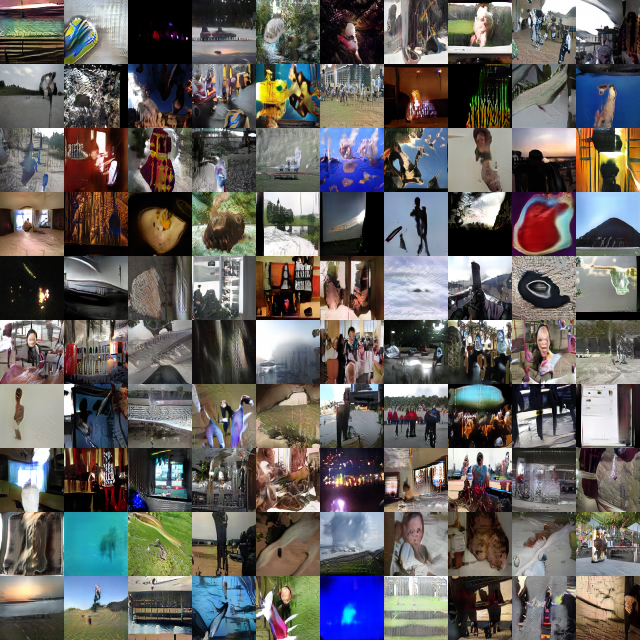
\includegraphics[width=\linewidth]{resultados/filtered_3chan.png}
   \caption{Muestras resultante del dataset YFCC100m filtrado de tres canales.}
  \label{fig:resultado_filtrado4}
\end{figure}


\chapter{Resultados del dataset YFCC100m}\label{apendice:sin_filtrar}
\begin{figure}[H]
\centering
 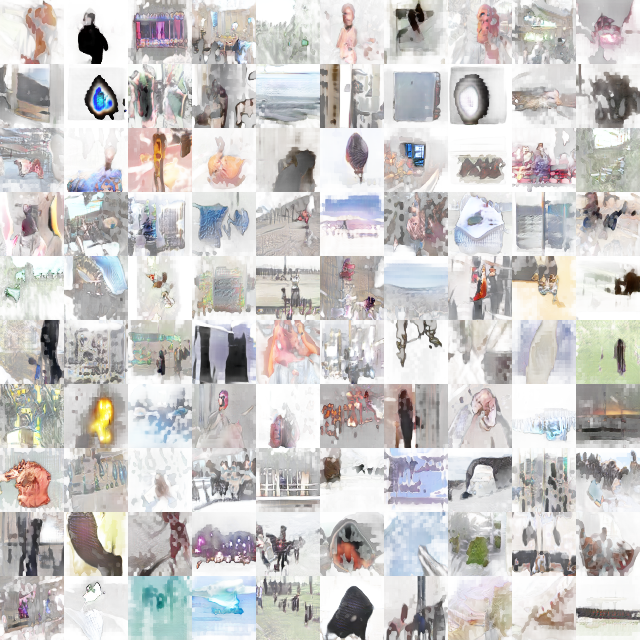
\includegraphics[width=\linewidth]{resultados/4chan_normal.png}
   \caption{Muestras resultante del dataset YFCC100m de cuatro canales.}
  \label{fig:resultado_sin_filtrar1}
\end{figure}

\begin{figure}[h]
\centering
 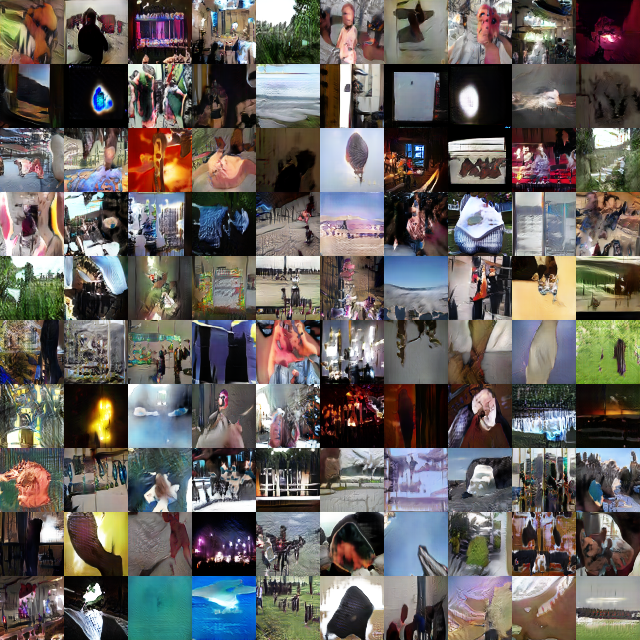
\includegraphics[width=\linewidth]{resultados/4chan_noalpha.png}
   \caption{Muestras resultante del dataset YFCC100m de cuatro canales sin el canal alpha.}
  \label{fig:resultado_sin_filtrar2}
\end{figure}

\begin{figure}[h]
\centering
 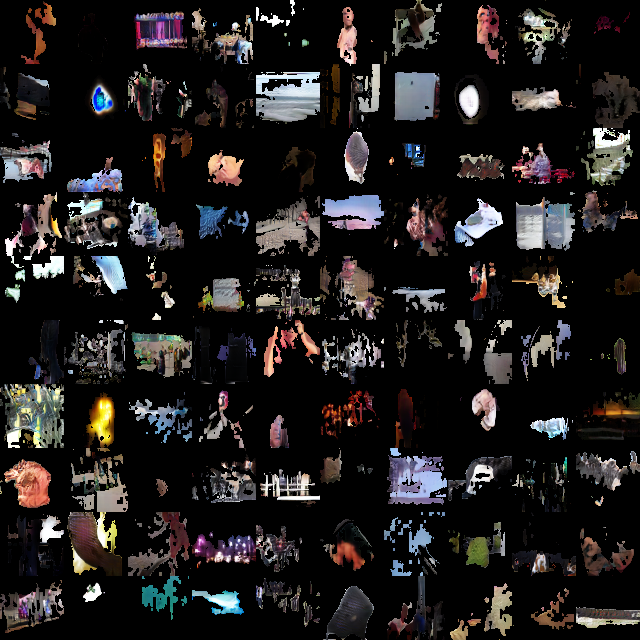
\includegraphics[width=\linewidth]{resultados/4chan_mask.png}
   \caption{Muestras resultante del dataset YFCC100m de cuatro canales aplicando una máscara negra sobre el fondo del objeto enfocado.}
  \label{fig:resultado_sin_filtrar3}
\end{figure}

\begin{figure}[h]
\centering
 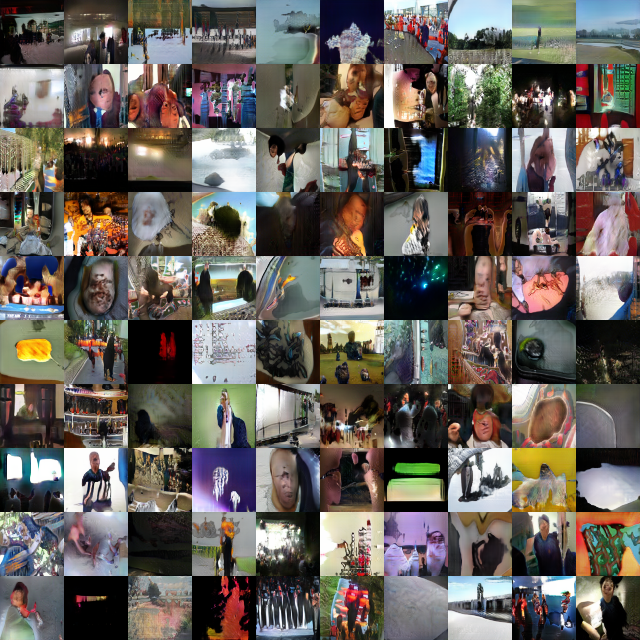
\includegraphics[width=\linewidth]{resultados/3chan.png}
   \caption{Muestras resultante del dataset YFCC100m de tres canales.}
  \label{fig:resultado_sin_filtrar4}
\end{figure}



\printbibliography


%%\bibliography{references}{}
%%\bibliographystyle{plain}
\end{document}
